\documentclass[10pt]{beamer}
\usetheme{metropolis}
% all imports
\usepackage{lmodern}
\usepackage[utf8]{inputenc}
\usepackage[T1]{fontenc}
\usepackage{appendixnumberbeamer}
\usepackage{hyperref}
\usepackage{booktabs}
\usepackage{bm}
\usepackage[scale=2]{ccicons}
\usepackage[outputdir=build]{minted}
\usepackage{pgfplots}
\usepackage{array,colortbl,xcolor}
\usepgfplotslibrary{dateplot}
\usepackage{setspace}
\usepackage{etoolbox}
\usepackage{xspace}
\usepackage{tikz}
\usetikzlibrary{shapes,arrows,positioning,fit,backgrounds}
\usepackage{tkz-euclide}

\AtBeginEnvironment{quote}{\singlespacing}


\AtBeginEnvironment{quote}{\singlespacing}

% new commands
\newcommand{\themename}{\textbf{\textsc{metropolis}}\xspace}
\newcommand{\vect}[1]{\bm{#1}}
\newcommand{\myprime}[1]{{#1}^{\prime}}
\newcommand{\grad}[2]{\nabla_{#1} {#2}}
\newcommand{\dotp}[2]{{#1}^{\top}{#2}}
\newcommand{\dotpPright}[2]{{#1}^{\top}\left({#2}\right)}
\newcommand{\outerp}[2]{\left({#1}\right){#2}^{\top}}
\newcommand{\Jacobian}[2]{\frac{\partial #1}{\partial #2}}
\newcommand{\Vocab}{\mathbb{V}}
\DeclareMathOperator*{\argmin}{arg\,min}
\DeclareMathOperator*{\argmax}{arg\,max}
\DeclareMathOperator{\E}{\mathbb{E}}

% definitions
\definecolor{blue}{RGB}{159, 192, 176}
\definecolor{blue2}{RGB}{38,139,210}
\definecolor{green}{RGB}{160, 227, 127}
\definecolor{green2}{RGB}{132, 164, 76}
\definecolor{orange}{RGB}{243, 188, 125}
\definecolor{red}{RGB}{253, 123, 84}
\definecolor{nephritis}{RGB}{39, 174, 96}
\definecolor{emerald}{RGB}{46, 204, 113}
\definecolor{turquoise}{RGB}{39, 174, 96}
\definecolor{green-sea}{RGB}{22, 160, 133}
\definecolor{base02}{RGB}{7,54,66}
\definecolor{base03}{RGB}{0,43,54}
\definecolor{cyan}{RGB}{42,161,152}

% Tikzstyles for Computation Graphs

% nodes
\tikzstyle{noop} = [circle, draw=none, fill=red, minimum size = 10pt]
\tikzstyle{op} = [circle, draw=red, line width=1.5pt, fill=red!70, text=black, text centered, font=\bf \normalsize, minimum size = 25pt]
\tikzstyle{op2} = [circle, draw=orange, line width=1.5pt, fill=orange!70, text=black, text centered, font=\bf \normalsize, minimum size = 25pt]
\tikzstyle{op3} = [circle, draw=orange, line width=1.5pt, fill=orange!70, text=black, text centered, font=\bf \scriptsize, minimum size = 7pt]
\tikzstyle{placeholder} = [circle, draw=red, line width=1.5pt, fill=red!30, text=black, text centered, font=\bf  \normalsize, minimum size = 25pt]
\tikzstyle{state} = [circle, draw=blue, line width=1.5pt, fill=blue!70, text=black, text centered, font=\bf \normalsize, minimum size = 25pt]
\tikzstyle{gradient} = [circle, draw=nephritis, line width=1.5pt, fill=nephritis!60, text=black, text centered, font=\bf \normalsize, minimum size = 25pt]
\tikzstyle{gradient2} = [circle, draw=green2, line width=1.5pt, fill=green2!60, text=black, text centered, font=\bf \normalsize, minimum size = 25pt]
\tikzstyle{textonly} = [draw=none, fill=none, text centered, font=\bf \normalsize]

% edges
% \tikzstyle{tedge}  = [draw, thick, >=stealth, ->]
\tikzstyle{tedge}  = [draw, thick, >=latex, ->]
\tikzstyle{tedge_dashed}  = [draw, thick, >=latex, ->, dashed]

% namedscope
\tikzstyle{namedscope} = [circle, draw=orange, line width=1.5pt, fill=orange!60, align=center, inner sep=0pt]

% \tikzstyle{container} = [draw=none, rectangle, dotted, inner ysep=1.5em]
% \tikzstyle{novertex} = [draw=none, fill=none, text centered]
% \tikzstyle{predicate} = [ellipse, draw, thick, text centered, rounded corners, minimum size=30pt]
% \tikzstyle{aux} = [rectangle, draw, thick, text centered, rounded corners, minimum size=30pt]
% \tikzstyle{ledge}  = [draw, dashed, thick, >=stealth, ->]
% \tikzstyle{pedge}  = [draw, thick, >=stealth, ->]



\title{Primeiros passos de Deep Learning em Python}
\date{\today}

\author{
  Antonio Abello\\
  \url{https://github.com/Abello966}\\\vspace{0.4 cm}
  \and\\ 
  Felipe Salvatore\\
  \url{https://felipessalvatore.github.io/}
  \vspace{0.4 cm}
}

\institute{\textbf{IME-USP}: Instituto de Matemática e Estatística, Universidade de São Paulo}


\begin{document}
\nocite{DeepLearningbook}
\nocite{xiao2017/online}
\maketitle

\section{Introdução}
\begin{frame}[fragile]{Por que Deep Learning?}
\fontsize{12pt}{12}
\begin{itemize}
	\item \textbf{Engenharia de Features} (\alert{Feature Engineering}): como extrair informação relevante dos dados?
    \vspace{2em}
    \item \textbf{Representação de features}: como representar a informação para facilitar as tarefas?
\end{itemize}
\end{frame}
\begin{frame}[fragile]{Feature Engineering - Imagens}
\begin{center}
\begin{tikzpicture}
\node (original) at (1, 6) 
	{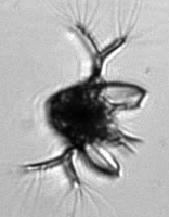
\includegraphics[width=.15\textwidth]{images/original.png}};
\node (segmented) at (5, 6)
	{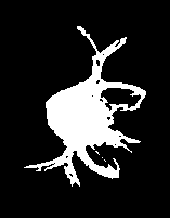
\includegraphics[width=.15\textwidth]{images/segmented.png}};
	
\node (circled) at (0, 3)
	{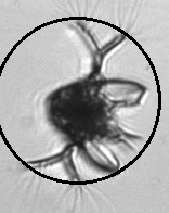
\includegraphics[width=.15\textwidth]{images/circled.png}};
\node (rected) at (3, 3)
	{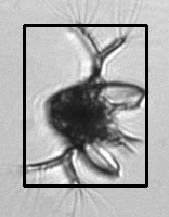
\includegraphics[width=.15\textwidth]{images/rected.png}};
\node (ellipsed) at (6, 3)
	{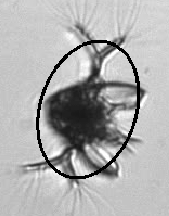
\includegraphics[width=.15\textwidth]{images/ellipsed.png}};
	
\draw[->, thick] (original.east) -- (segmented.west);
\draw[->, thick] (segmented.south) -- (circled.north);
\draw[->, thick] (segmented.south) -- (rected.north);
\draw[->, thick] (segmented.south) -- (ellipsed.north);
\draw[->, thick] (circled.south) -- (0.5, 0.7);
\draw[->, thick] (rected.south) -- (3, 0.7);
\draw[->, thick] (ellipsed.south) -- (5.5, 0.7);

\foreach \i in {0,...,12}
{
	\pgfkeys{/pgf/number format/.cd,fixed,precision=0}
	\pgfmathsetmacro\myvalue{abs(rand) * 10}
	\draw[fill=blue!45!white] (0.5 * \i, 0) rectangle (0.5 + 0.5 * \i, 0.5) node[pos=.5]{\pgfmathprintnumber\myvalue};
}
\end{tikzpicture}
\end{center}
\end{frame}

\begin{frame}[fragile]{Feature Engineering}
\fontsize{12pt}{12}
\begin{itemize}
	\item Conhecimento especializado
    \vspace{1em}
	\item Geralmente não aplicável a diferentes domínios
    \vspace{1em}
    \item Difícil de avaliar
    \vspace{1em}
	\item "Humano, demasiado humano"
\end{itemize}
\end{frame}

\begin{frame}[fragile]{Espaço de representação - Problemas}
\begin{figure}
	\centering
		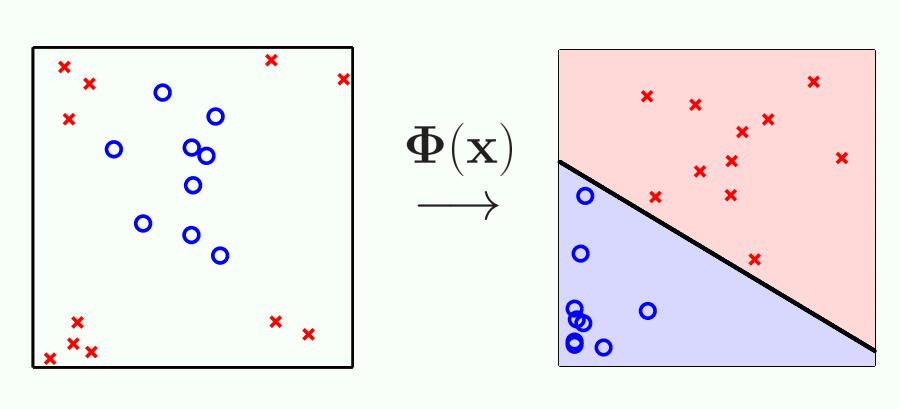
\includegraphics[height=0.35\textwidth]		{images/nonlinear_transform.png}
    \caption{Transformação $\Phi$ possibilita classificação por classificador linear \cite{MostafaLD2012}}
\end{figure}
\begin{itemize}
	\item Relação entre features: compor diferentes features matematicamente leva a informações úteis não aproveitadas
    \item Transformações não-lineares: podem ajudar, mas como escolher?
\end{itemize}
\end{frame}

\begin{frame}[fragile]{Deep Learning}
	\begin{exampleblock}{}
   		"The solution is to allow computers to \alert{learn from experience} and understand the world in terms of a hierarchy of concepts, with each concept defined through its relation to simpler concepts. (...) This approach \alert{avoids the need for human operators to formally specify} all the knowledge that the computer needs. (...) If we draw a graph showing how these concepts are built on top of each other, the \alert{graph is deep}, with many layers. For this reason, we call this approach \alert{deep learning}."\\
        
I. Goodfellow, Y. Bengio, A. Courville -- \textbf{Deep Learning} (2017)
    \end{exampleblock}
\end{frame}

\section{Representação gráfica}

\begin{frame}[fragile]{Perceptron}
\begin{figure}[ht!]
\centering

\scalebox{1.15}{
\begin{tikzpicture}[auto]

% operations =============================
\node[op] (x2) {$x_2$};
\node[op, above=40pt of x2] (x1) {$x_1$};
\node[op, below=40pt of x2] (x3) {$x_3$};
\node[op, right=60pt of x2] (vk) {$v$};
\node[op, right=40pt of vk] (yk) {$\hat{y}$};
\node[textonly, below right=20pt of x3] (Synaptic) {Synaptic link};
\node[textonly, below right=50pt of vk] (Activation) {Activation link};
\node[textonly, above right=28pt and -46pt of yk] (f) {$\hat{y} = f(\vect{x};\vect{\theta})= g\left(\sum_{i=1}^{3} \theta_ix_i\right)$};


% edges
\path[tedge] (x1) edge node[above=1.8pt] {$\theta_{1}$} (vk);
\path[tedge] (x2) edge node[above=0.2pt] {$\theta_{2}$} (vk);
\path[tedge] (x3) edge node[above=3.8pt] {$\theta_{3}$} (vk);
\path[tedge] (vk) edge node[above=1pt] {{\Large$g$}}  (yk) ;

% info edges
\draw[orange!120, line width=1mm]  (Synaptic) to [out=150,in=0] (x3);
\draw[orange!120, line width=1mm] (Synaptic) to [out=150,in=-100] (vk);

\draw[orange!120, line width=1mm]  (Activation) to [out=170,in=-40] (vk);
\draw[orange!120, line width=1mm] (Activation) to [out=170,in=-100] (yk);



\end{tikzpicture}
} % scalebox
\end{figure}

\end{frame}

\begin{frame}[fragile]{Revisão: função sigmoide}
\begin{figure}[ht!]
\centering

\scalebox{1.0}{
\begin{tikzpicture}
    \begin{axis}%
    [
        grid=major,     
        xmin=-6,
        xmax=6,
        axis x line=bottom,
        ytick={0,.5,1},
        ymax=1,
        axis y line=middle,
    ]
        \addplot%
        [	orange!180,
        	ultra thick,
%             blue,%
            mark=none,
            samples=100,
            domain=-6:6,
        ]
        (x,{1/(1+exp(-x))});
    \end{axis}
\node[textonly] (sigmoid) at (8.75,2.8) {{\Large$\sigma(x) = \frac{1}{1 + e^{-x}}$}};
\end{tikzpicture}
} % scalebox
\end{figure}
\end{frame}

\begin{frame}[fragile]{ReLU: Rectified Linear Units}
\begin{figure}[ht!]
\centering

\scalebox{1.0}{
\begin{tikzpicture}
    \begin{axis}%
    [
        grid=major,     
        xmin=-6,
        xmax=6,
        axis x line=bottom,
        ytick={0},
        ymax=10,
        axis y line=middle,
    ]
        \addplot%
        [	orange!180,
        	ultra thick,
%             blue,%
            mark=none,
            samples=100,
            domain=-6:6,
        ]
        (x,{max(x,0)});
    \end{axis}
\node[textonly] (relu) at (8.95,2.8) {{\Large$g(x) = max\{0,x\}$}};
\end{tikzpicture}
} % scalebox
\end{figure}
\end{frame}

\begin{frame}[fragile]{Revisão: função softmax}
\begin{figure}[ht!]
\centering

\scalebox{1.3}{
\begin{tikzpicture}[auto]

% operations =============================

% nodes
\node[textonly] (logits) {$\begin{bmatrix}3.82\\5.35\\1.44\\-1.26\\2.71 \\1.98\end{bmatrix}$};
\node[textonly, right=60pt of logits] (softmax) {$\begin{bmatrix}0.16115195\\0.74422819\\0.01491471\\0.00100235\\0.05310907 \\0.02559374\end{bmatrix}$};
\node[textonly, below=15pt of logits] (inv1) {};
\node[textonly, right=10pt of inv1] (softmax_eq) {{\Large$softmax(x) = \frac{e^{x}}{\sum e^{x}}$}};



% edges
\path[tedge] (logits) edge node[above=1pt] {{\Large softmax}} (softmax);
\end{tikzpicture}
} % scalebox
\end{figure}

\end{frame}

\begin{frame}[fragile]{Rede neural: versão antiga}
\begin{figure}[ht!]
\centering

\scalebox{0.7}{
\begin{tikzpicture}[auto]

% operations =============================

% input layer
\node[op] (x5) {$x_5$};
\node[op, above=2.5pt of x5] (x4) {$x_4$};
\node[op, above=2.5pt of x4] (x3) {$x_3$};
\node[op, above=2.5pt of x3] (x2) {$x_2$};
\node[op, above=2.5pt of x2] (x1) {$x_1$};
\node[op, below=2.5pt of x5] (x6) {$x_6$};
\node[op, below=2.5pt of x6] (x7) {$x_7$};
\node[op, below=2.5pt of x7] (x8) {$x_8$};
\node[op, below=2.5pt of x8] (x9) {$x_9$};
\node[op, below=2.5pt of x9] (x10) {$x_{10}$};

% hidden layer
\node[op,  right=130pt of x5] (v2) {$v_2$};
\node[op, below=2.5pt of v2] (v3) {$v_3$};
\node[op, below=2.5pt of v3] (v4) {$v_4$};
\node[op, above=2.5pt of v2] (v1) {$v_1$};

\node[op,  right=40pt of v2] (h2) {$h_2$};
\node[op, below=2.5pt of h2] (h3) {$h_3$};
\node[op, below=2.5pt of h3] (h4) {$h_4$};
\node[op, above=2.5pt of h2] (h1) {$h_1$};


% output layer
\node[op,  right=60pt of h2] (z1) {$z_1$};
\node[op,  right=60pt of h3] (z2) {$z_2$};

\node[op,  right=50pt of z1] (y1) {$\hat{y}_1$};
\node[op,  right=50pt of z2] (y2) {$\hat{y}_2$};


% edges input layer to hidden
\path[tedge] (x1) -- (v1);
\path[tedge] (x1) -- (v2);
\path[tedge] (x1) -- (v3);
\path[tedge] (x1) -- (v4);

\path[tedge] (x2) -- (v1);
\path[tedge] (x2) -- (v2);
\path[tedge] (x2) -- (v3);
\path[tedge] (x2) -- (v4);

\path[tedge] (x3) -- (v1);
\path[tedge] (x3) -- (v2);
\path[tedge] (x3) -- (v3);
\path[tedge] (x3) -- (v4);

\path[tedge] (x4) -- (v1);
\path[tedge] (x4) -- (v2);
\path[tedge] (x4) -- (v3);
\path[tedge] (x4) -- (v4);

\path[tedge] (x5) -- (v1);
\path[tedge] (x5) -- (v2);
\path[tedge] (x5) -- (v3);
\path[tedge] (x5) -- (v4);

\path[tedge] (x6) -- (v1);
\path[tedge] (x6) -- (v2);
\path[tedge] (x6) -- (v3);
\path[tedge] (x6) -- (v4);

\path[tedge] (x7) -- (v1);
\path[tedge] (x7) -- (v2);
\path[tedge] (x7) -- (v3);
\path[tedge] (x7) -- (v4);

\path[tedge] (x8) -- (v1);
\path[tedge] (x8) -- (v2);
\path[tedge] (x8) -- (v3);
\path[tedge] (x8) -- (v4);

\path[tedge] (x9) -- (v1);
\path[tedge] (x9) -- (v2);
\path[tedge] (x9) -- (v3);
\path[tedge] (x9) -- (v4);

\path[tedge] (x10) -- (v1);
\path[tedge] (x10) -- (v2);
\path[tedge] (x10) -- (v3);
\path[tedge] (x10) -- (v4);

% edges hidden to hidden
\path[tedge] (v1) edge node[above=1pt] {{\Large$\sigma$}}  (h1) ;
\path[tedge] (v2) edge node[above=1pt] {{\Large$\sigma$}}  (h2) ;
\path[tedge] (v3) edge node[above=1pt] {{\Large$\sigma$}}  (h3) ;
\path[tedge] (v4) edge node[above=1pt] {{\Large$\sigma$}}  (h4) ;

% edges hidden to output
\path[tedge] (h1) -- (z1);
\path[tedge] (h1) -- (z2);

\path[tedge] (h2) -- (z1);
\path[tedge] (h2) -- (z2);

\path[tedge] (h3) -- (z1);
\path[tedge] (h3) -- (z2);

\path[tedge] (h4) -- (z1);
\path[tedge] (h4) -- (z2);

% edges output to output
\path[tedge] (z1) edge node[above=1pt] {{\Large softmax}}  (y1) ;
\path[tedge] (z2) edge node[above=1pt] {{\Large softmax}}  (y2) ;




\end{tikzpicture}
} % scalebox
\end{figure}

\end{frame}

\begin{frame}[fragile]{Rede neural: versão antiga}
\begin{figure}[ht!]
\centering

\scalebox{0.7}{
\begin{tikzpicture}[auto]

% operations =============================

% input layer
\node[op] (x5) {};
\node[op, above=2.5pt of x5] (x4) {};
\node[op, above=2.5pt of x4] (x3) {};
\node[op, above=2.5pt of x3] (x2) {};
\node[op, above=2.5pt of x2] (x1) {};
\node[op, below=2.5pt of x5] (x6) {};
\node[op, below=2.5pt of x6] (x7) {};
\node[op, below=2.5pt of x7] (x8) {};
\node[op, below=2.5pt of x8] (x9) {};
\node[op, below=2.5pt of x9] (x10) {};

\node[textonly, above=2.5pt of x1] (x) {{\LARGE$\vect{x}$}};
\node[textonly, below=4.5pt of x10] (input) {{\large Input layer}};

% hidden layer
\node[op,  right=130pt of x5] (h2) {};
\node[op, below=2.5pt of h2] (h3) {};
\node[op, below=2.5pt of h3] (h4) {};
\node[op, above=2.5pt of h2] (h1) {};

\node[textonly, above=2.5pt of h1] (h) {{\LARGE$\vect{h}$}};
\node[textonly, below=4.5pt of h4] (hidden) {{\large Hidden layer}};

% output layer
\node[op,  right=60pt of h2] (y1) {};
\node[op,  right=60pt of h3] (y2) {};

\node[textonly, above=2.5pt of y1] (y) {{\LARGE$\hat{\vect{y}}$}};
\node[textonly, below=4.5pt of y2] (output) {{\large Output layer}};

% edges input layer to hidden
\path[tedge] (x1) -- (h1);
\path[tedge] (x1) -- (h2);
\path[tedge] (x1) -- (h3);
\path[tedge] (x1) -- (h4);

\path[tedge] (x2) -- (h1);
\path[tedge] (x2) -- (h2);
\path[tedge] (x2) -- (h3);
\path[tedge] (x2) -- (h4);

\path[tedge] (x3) -- (h1);
\path[tedge] (x3) -- (h2);
\path[tedge] (x3) -- (h3);
\path[tedge] (x3) -- (h4);

\path[tedge] (x4) -- (h1);
\path[tedge] (x4) -- (h2);
\path[tedge] (x4) -- (h3);
\path[tedge] (x4) -- (h4);

\path[tedge] (x5) -- (h1);
\path[tedge] (x5) -- (h2);
\path[tedge] (x5) -- (h3);
\path[tedge] (x5) -- (h4);

\path[tedge] (x6) -- (h1);
\path[tedge] (x6) -- (h2);
\path[tedge] (x6) -- (h3);
\path[tedge] (x6) -- (h4);

\path[tedge] (x7) -- (h1);
\path[tedge] (x7) -- (h2);
\path[tedge] (x7) -- (h3);
\path[tedge] (x7) -- (h4);

\path[tedge] (x8) -- (h1);
\path[tedge] (x8) -- (h2);
\path[tedge] (x8) -- (h3);
\path[tedge] (x8) -- (h4);

\path[tedge] (x9) -- (h1);
\path[tedge] (x9) -- (h2);
\path[tedge] (x9) -- (h3);
\path[tedge] (x9) -- (h4);

\path[tedge] (x10) -- (h1);
\path[tedge] (x10) -- (h2);
\path[tedge] (x10) -- (h3);
\path[tedge] (x10) -- (h4);

% edges hidden to output
\path[tedge] (h1) -- (y1);
\path[tedge] (h1) -- (y2);

\path[tedge] (h2) -- (y1);
\path[tedge] (h2) -- (y2);

\path[tedge] (h3) -- (y1);
\path[tedge] (h3) -- (y2);

\path[tedge] (h4) -- (y1);
\path[tedge] (h4) -- (y2);



\end{tikzpicture}
} % scalebox
\end{figure}

\end{frame}

%\begin{frame}[fragile]{Rede neural: versão antiga}
%\begin{center}
%\begin{figure}[ht!]
\centering

\scalebox{0.7}{
\begin{tikzpicture}[auto]

% operations =============================

% input layer
\node[op] (x5) {};
\node[op, above=2.5pt of x5] (x4) {};
\node[op, above=2.5pt of x4] (x3) {};
\node[op, above=2.5pt of x3] (x2) {};
\node[op, above=2.5pt of x2] (x1) {};
\node[op, below=2.5pt of x5] (x6) {};
\node[op, below=2.5pt of x6] (x7) {};
\node[op, below=2.5pt of x7] (x8) {};
\node[op, below=2.5pt of x8] (x9) {};
\node[op, below=2.5pt of x9] (x10) {};

\node[textonly, above=2.5pt of x1] (x) {{\LARGE$\vect{x}$}};
\node[textonly, below=4.5pt of x10] (input) {{\large Input layer}};

% hidden layer
\node[op,  right=130pt of x5] (h2) {};
\node[op, below=2.5pt of h2] (h3) {};
\node[op, below=2.5pt of h3] (h4) {};
\node[op, above=2.5pt of h2] (h1) {};

\node[textonly, above=2.5pt of h1] (h) {{\LARGE$\vect{h}$}};
\node[textonly, below=4.5pt of h4] (hidden) {{\large Hidden layer}};

% output layer
\node[op,  right=60pt of h2] (y1) {};
\node[op,  right=60pt of h3] (y2) {};

\node[textonly, above=2.5pt of y1] (y) {{\LARGE$\hat{\vect{y}}$}};
\node[textonly, below=4.5pt of y2] (output) {{\large Output layer}};

% edges input layer to hidden
\draw[line width=0.5mm] (x1) -- (hidden);
\draw[line width=0.5mm] (x10) -- (h);

% edges hidden to output
\draw [line width=0.5mm]  (h1) -- (output);
\draw [line width=0.5mm]  (h4) -- (y);

\end{tikzpicture}
} % scalebox
\end{figure}

%\end{center}
%\end{frame}

\begin{frame}[fragile]{Grafo de computação}
\begin{figure}[ht!]
\centering

\scalebox{1.3}{
\begin{tikzpicture}[auto]

% operations =============================

% nodes
\node[op] (W1) {$\vect{W}$};
\node[textonly, below=20pt of W1] (inv1) {};
\node[op, below=40pt of W1] (x1) {$\vect{x}$};
\node[op, right=30.5pt of inv1] (v1) {matmul};
\node[op, right=120pt of W1] (W2) {$\vect{W}$};
\node[textonly, below=20pt of W2] (inv2) {};
\node[op, below=40pt of W2] (x2) {$\vect{x}$};
\node[op, right=30.5pt of inv2] (v2) {$\vect{v}$};
\node[textonly, left=1.5pt of v2] (matmtul) {matmul};
\node[textonly, left=40pt of inv2] (inv3) {};
\node[textonly, below=50.5pt of inv3] (result) {{\large $\vect{v} = \vect{W} \vect{x} $}};

% edges
\path[tedge] (W1) -- (v1);
\path[tedge] (x1) -- (v1);
\path[tedge] (W2) -- (v2);
\path[tedge] (x2) -- (v2);

\end{tikzpicture}
} % scalebox
\end{figure}

\end{frame}

\begin{frame}[fragile]{Grafo de computação}
\begin{figure}[ht!]
\centering

\scalebox{1.15}{
\begin{tikzpicture}[auto]

% operations =============================

% nodes
\node[op] (W1) {$\vect{W}_{1}$};
\node[textonly, below=40pt of W1] (inv1) {};
\node[op, below=20pt of inv1] (x) {$\vect{x}$};
\node[op, right=30.5pt of inv1] (v) {$\vect{v}$};
\node[textonly, left=1.5pt of v] (matmtul1) {matmul};
\node[op, right=35pt of v] (h) {$\vect{h}$};
\node[op, right=110pt of W1] (W2) {$\vect{W}_{2}$};
\node[op, right=35pt of h] (z) {$\vect{z}$};
\node[op, right=55pt of z] (y) {$\hat{\vect{y}}$};
\node[textonly, above left=1.5pt of z] (matmtul2) {matmul};


% edges
\path[tedge] (W1) -- (v);
\path[tedge] (x) -- (v);
\path[tedge] (v) edge node[above=1pt] {{\Large$\sigma$}} (h);
\path[tedge] (z) edge node[above=1pt] {{\Large softmax}}  (y);
\path[tedge] (W2) -- (z);
\path[tedge] (h) -- (z);


\end{tikzpicture}
} % scalebox
\end{figure}

\end{frame}

\begin{frame}[fragile]{Grafo no Tensorflow}
\begin{minted}[linenos]{python}
import tensorflow as tf
import numpy as np

input_shape = [10,1]
input_to_hidden_shape = [4,10]
hidden_to_output_shape = [2,4]

W1init = np.zeros(input_to_hidden_shape,
                  dtype="float32")
W2init = np.zeros(hidden_to_output_shape,
                  dtype="float32")
\end{minted}
\end{frame}


\begin{frame}[fragile]{Grafo no Tensorflow}
\begin{minted}[linenos]{python}
graph = tf.Graph() 
with graph.as_default():
    x = tf.placeholder(shape=input_shape,
                       dtype="float32") 
    W1 = tf.get_variable(initializer=W1init)
    v = tf.matmul(W1, x)
    h = tf.sigmoid(v)
    W2 = tf.get_variable(initializer=W2init)
    z = tf.matmul(W2, h)
    yhat = tf.nn.softmax(z)
\end{minted}
\end{frame}


\begin{frame}[fragile]{Visualizando o grafo no Tensorboard}
\begin{center}
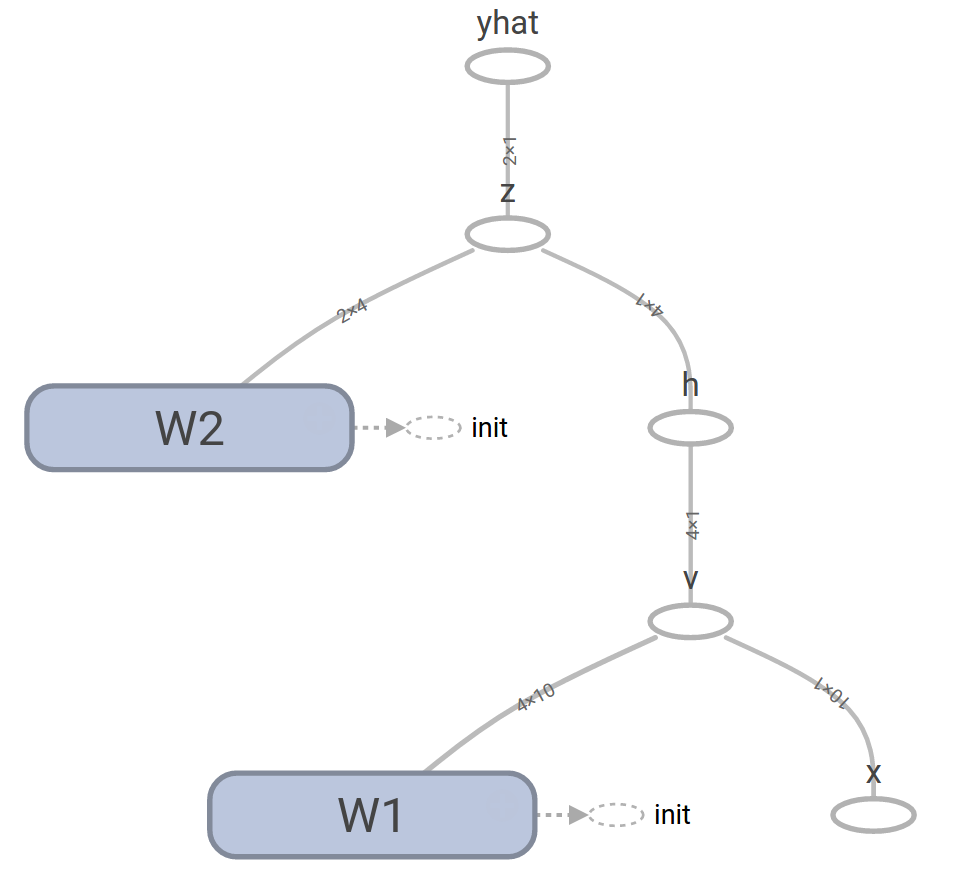
\includegraphics[scale=0.255]{images/basic_tf_graph.png}
\end{center}
\end{frame}

\begin{frame}[fragile]{Grafo de computação}
\begin{figure}[ht!]
\centering

\scalebox{1.2}{
\begin{tikzpicture}[auto]

% operations =============================

% nodes on the left
\node[op] (W1) {$\vect{W}_{1}$};
\node[textonly, below=20pt of W1] (inv1) {};
\node[op, right=30pt of inv1] (v) {$\vect{v}$};
\node[op, below right=30.5pt of v] (x) {$\vect{x}$};
\node[op, above=30.5pt of v] (hprime) {$\vect{h}^{\prime}$};
\node[textonly, above right=2pt of hprime] (h) {{\LARGE$\vect{h}$}};


%% namedscope in the left
\begin{scope}[on background layer]
\coordinate (p1) at (hprime.north);
\coordinate (p2) at (v.south east);
\coordinate (p3) at (W1.west);
\tkzCircumCenter(p1,p2,p3)
\tkzGetPoint{O}
\tkzDrawCircle[draw=orange, line width=1.5pt, fill=orange!60](O,p1)
\end{scope}

% edges on the left
\path[tedge] (W1) -- (v);
\path[tedge] (x) -- (v);
\path[tedge] (v) -- (hprime);

% nodes on the right
\node[op, right=30pt of x] (hh) {$\vect{h}$};
\node[op, above right=30.5pt of hh] (z) {$\vect{z}$};
\node[op, above=30.5pt of z] (yprime) {$\vect{y}^{\prime}$};
\node[textonly, right=30pt of z] (inv2) {};
\node[op, above=20pt of inv2] (W2) {$\vect{W}_{2}$};
\node[textonly, above left=1pt of yprime] (yhat) {{\LARGE$\hat{\vect{y}}$}};


%% namedscope in the right
\begin{scope}[on background layer]
\coordinate (p1) at (yprime.north);
\coordinate (p2) at (W2.north east);
\coordinate (p3) at (z.south west);
\tkzCircumCenter(p1,p2,p3)
\tkzGetPoint{O}
\tkzDrawCircle[draw=orange, line width=1.5pt, fill=orange!60](O,p1)
\end{scope}



% edges on the right
\path[tedge] (W2) -- (z);
\path[tedge] (hh) -- (z);
\path[tedge] (z) -- (yprime);


\end{tikzpicture}
} % scalebox
\end{figure}

\end{frame}

\begin{frame}[fragile]{Grafo de computação}
\begin{figure}[ht!]
\centering

\scalebox{1.5}{
\begin{tikzpicture}[auto]

% operations =============================
\node[op] (h) {$\vect{h}$};
\node[op, above=30pt of h] (y) {$\hat{\vect{y}}$};
\node[op, below=30pt of h] (x) {$\vect{x}$};


% edges
\path[tedge] (x) -- (h);
\path[tedge] (h) -- (y);

\end{tikzpicture}
} % scalebox
\end{figure}

\end{frame}


\begin{frame}[fragile]{Visualizando o grafo no Tensorboard}
\begin{center}
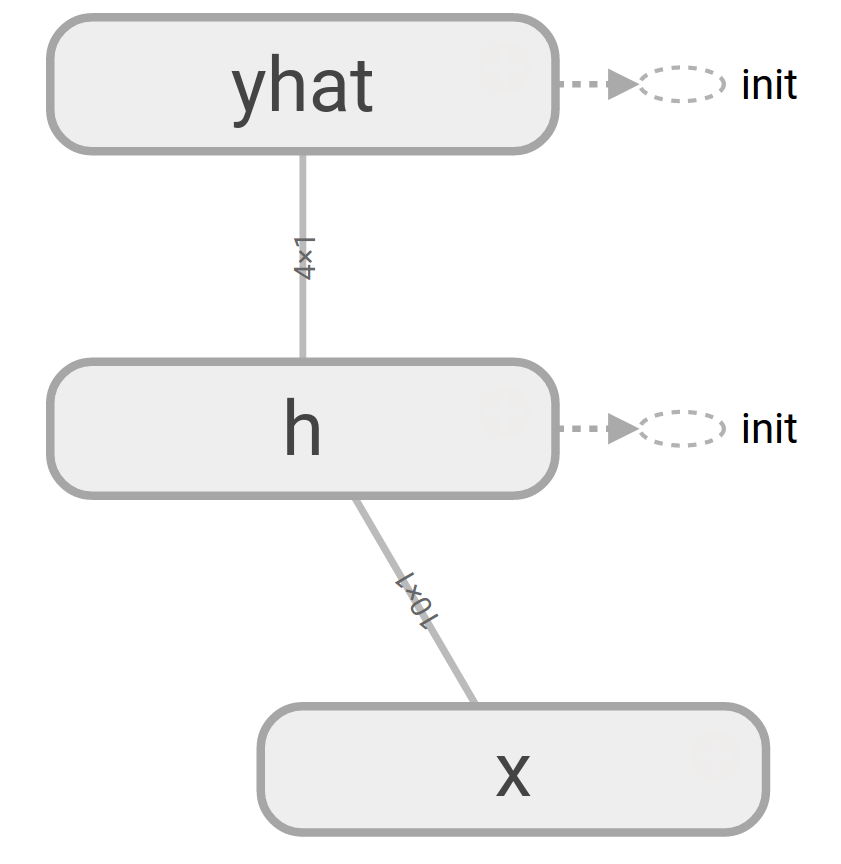
\includegraphics[scale=0.27]{images/abstract_tf_graph1.png}
\end{center}
\end{frame}

\begin{frame}[fragile]{Visualizando o grafo no Tensorboard}
\begin{center}
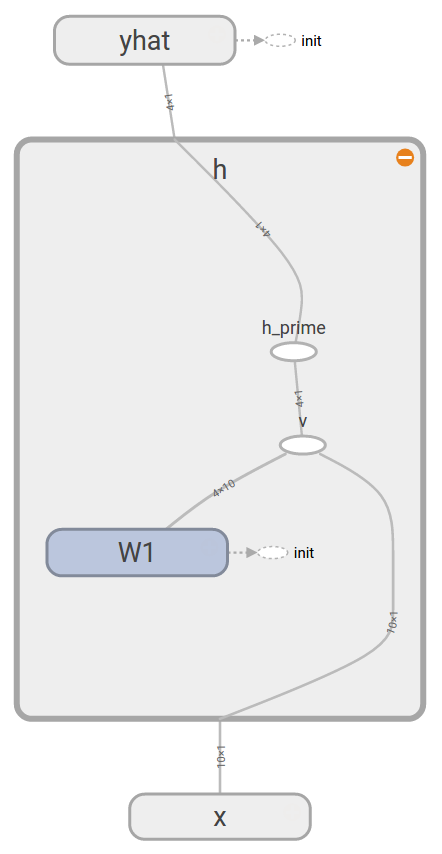
\includegraphics[scale=0.26]{images/abstract_tf_graph2.png}
\end{center}
\end{frame}


\section{DFN - Deep Feedforward Networks}


\begin{frame}{Deep Feedforward Networks}

\alert{Deep Feedforward Networks} são também chamadas de \alert{feedforward neural networks}, \alert{multilayer perceptrons}, ou, em bom português, \alert{redes neurais}.\\


Uma rede neural $\hat{\vect{y}} = f(\vect{x}; \vect{\theta})$ é um modelo parametrizado de aprendizado de máquina. Esse modelo pode ser descrito como uma composição de funções, por exemplo:

\begin{equation*}
f(\vect{x}; \vect{\theta}) = f^{(2)}(f^{(1)}(\vect{x}; \vect{\theta}); \vect{\theta})
\end{equation*}
\end{frame}

\begin{frame}{Rede neural}
\begin{figure}[ht!]
\centering

\scalebox{1.5}{
\begin{tikzpicture}[auto]

% operations =============================
\node[op] (h) {$\vect{h}$};
\node[op, above=30pt of h] (y) {$\hat{\vect{y}}$};
\node[op, below=30pt of h] (x) {$\vect{x}$};
\node[textonly, right=76pt of h] (inv) {};
\node[textonly, above=16pt of inv] (f1) {$\hat{y} = f^{(2)}(f^{(1)}(\vect{x}; \vect{W}_1); \vect{W}_2)$};
\node[textonly, below=10pt of f1] (f2) {$\hat{y} = softmax( \vect{W}_2 (\sigma(\vect{W}_1\vect{x})))$};


% edges
\path[tedge] (x) edge [out=90,in=-90] node[right] {$\vect{W}_{1}$} (h);
\path[tedge] (h) edge [out=90,in=-90] node[right] {$\vect{W}_{2}$} (y);

\end{tikzpicture}
} % scalebox
\end{figure}

\end{frame}

\begin{frame}{Rede neural profunda}
\begin{figure}[ht!]
\centering

\scalebox{0.7}{
\begin{tikzpicture}[auto]

% operations =============================
\node[op] (h1) {$\vect{h}^{(1)}$};
\node[op, below=30pt of h1] (x) {$\vect{x}$};
\node[op, above=30pt of h1] (h2) {$\vect{h}^{(2)}$};
\node[textonly, above=20pt of h2] (hdots) {{\LARGE$\vdots$}};
\node[op, above=20pt of hdots] (hn) {$\vect{h}^{(n)}$};
\node[op, above=30pt of hn] (y) {$\hat{\vect{y}}$};

%invisible nodes
\node[textonly, above right=2pt of y] (yinv1) {};
\node[textonly, below right=2pt of y] (yinv2) {};
\node[textonly, right=26pt of y] (yinv3) {output layer};

\node[textonly, above right=2pt of hn] (hinv1) {};
\node[textonly, below right=2pt of h1] (hinv2) {};
\node[textonly, right=26pt of h2] (hinv3) {hidden layers};

\node[textonly, above right=2pt of x] (xinv1) {};
\node[textonly, below right=2pt of x] (xinv2) {};
\node[textonly, right=26pt of x] (xinv3) {input layer};


\visible<2->{\node[textonly, above left=0.1pt and 0.1pt of y] (d1) {};}
\visible<2->{\node[textonly, below left=0.1pt and 0.1pt of x] (d2) {};}
\visible<2->{\node[textonly, left=56pt of hdots] (d3) {{\large\alert{deep model}}};}


% edges
\path[tedge] (x) -- (h1);
\path[tedge] (h1) -- (h2);
\path[tedge] (h2) -- (hdots);
\path[tedge] (hdots) -- (hn);
\path[tedge] (hn) -- (y);

% visual aid edges
\draw[orange!120, line width=1mm]  (yinv3) to [out=180,in=-80] (yinv1);
\draw[orange!120, line width=1mm]  (yinv3) to [out=180,in=80] (yinv2);


\draw[orange!120, line width=1mm]  (hinv3) to [out=180,in=-80] (hinv1);
\draw[orange!120, line width=1mm]  (hinv3) to [out=180,in=80] (hinv2);


\draw[orange!120, line width=1mm]  (xinv3) to [out=180,in=-80] (xinv1);
\draw[orange!120, line width=1mm]  (xinv3) to [out=180,in=80] (xinv2);


\visible<2->{\draw[orange!180, line width=1mm]  (d3) to [out=0,in=180] (d1);}
\visible<2->{\draw[orange!180, line width=1mm]  (d3) to [out=0,in=180] (d2);}



\end{tikzpicture}
} % scalebox
\end{figure}

\end{frame}

\begin{frame}{Redes neurais são aproximadores universais}
\textbf{Teorema da aproximação universal} (\alert{universal approximation theorem}): qualquer função Borel mensurável pode ser aproximada por uma rede neural com pelo menos uma camada escondida, dado que as camadas escondidas tenham um tamanho suficiente.\\

Toda função definida num subconjunto fechado e limitado de $\mathbb{R}^{n}$ é Borel mensurável, então um grande número de funções são aproximáveis por uma rede neural.  
\end{frame}

\begin{frame}{Redes neurais são aproximadores universais}

Uma rede neural com apenas uma camada escondida é suficiente para representar qualquer função. \\

Mas essa única camada pode ser muito grande e apresentar problemas para generalização. \textbf{Empiricamente redes com profundidade maior apresentam melhores resultados para generalização}.
\end{frame}



\begin{frame}{Receita para aprendizado de máquina}
\begin{itemize}
\item Uma tarefa de aprendizado sobre algum dataset. \visible<2->{\alert{Fashion MNIST}}
\vspace{0.3cm}
\item Uma família de modelos. \visible<2->{\alert{DFN}}
\vspace{0.3cm}
\item Uma função de custo. \visible<2->{\alert{Entropia cruzada}}
\vspace{0.3cm}
\item Um algoritmo de otimização. \visible<2->{\alert{SGD}}
\end{itemize}
\end{frame}


\begin{frame}[fragile]{Fashion MNIST}
\begin{center}
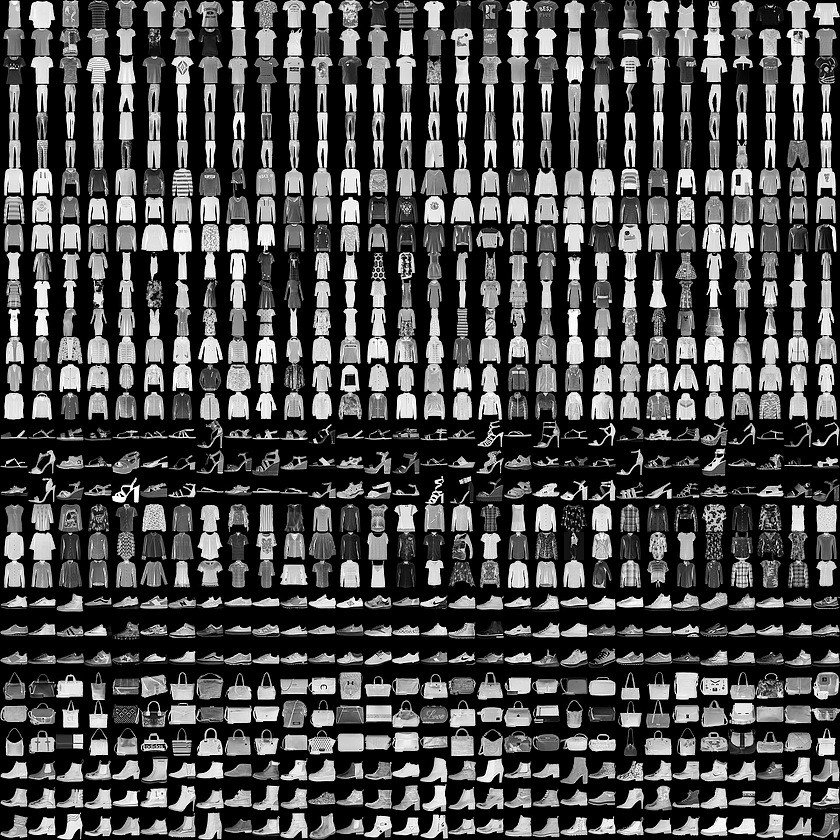
\includegraphics[scale=0.185]{images/fashion-mnist-general.png}
\end{center}
\begin{itemize}
\item Conjunto de treinamento: $60$k
\item Conjunto de teste: $10$k
\item Imagens: $28 \times 28$ tons de cinza.
\item 10 classes: (camiseta, vestido, sandália, ...)
\end{itemize}
\end{frame}

\begin{frame}{Fashion MNIST}
\begin{figure}[ht!]
\centering

\scalebox{1.05}{
\begin{tikzpicture}[auto]

% operations =============================

% nodes
\node (shirt)
    {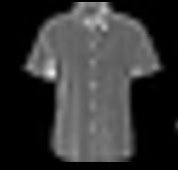
\includegraphics[width=.15\textwidth]{images/shirt.png}};
\node[textonly, below=1pt of shirt] (dimension0) {{\small$28\times 28$}};
\node[textonly, above right= 10pt and 90pt of shirt] (vector) {$\begin{bmatrix}0.34\\ \vdots \\0.06\end{bmatrix}$};
\node[textonly, above=1pt of vector] (x) {$\vect{x}$};
\node[textonly, below=1pt of vector] (dimension1) {{\small$784\times 1$}};

\node[textonly, below=30pt of vector] (y) {$y=1$};

\node[textonly, below=30pt of y] (one-hot) {$\begin{bmatrix}1\\ \vdots \\0\end{bmatrix}$};

\node[textonly, above=1pt of one-hot] (yvector) {$\vect{y}$};
\node[textonly, below=1pt of one-hot] (dimension2) {{\small$10\times 1$}};



% edges
\path[tedge, orange!120, line width=1mm]  (shirt) -- (vector);
\path[tedge, orange!120, line width=1mm] (shirt) -- (y);
\path[tedge, orange!120, line width=1mm] (shirt) -- (one-hot);



\end{tikzpicture}
} % scalebox
\end{figure}

\end{frame}

\begin{frame}{Princípio da máxima verossimilhança}
Vamos usar uma DFN para definir a distribuição $p(y| \vect{x};\vect{\theta})$. \\

Os parâmetros $\vect{\theta}$ vão ser adaptados de modo que  $p(y| \vect{x};\vect{\theta})$ seja a distribuição mais adequada para os dados
\begin{equation*}
(\vect{x}^{(1)},y^{(1)}), \dots, (\vect{x}^{(N)},y^{(N)})
\end{equation*}
\end{frame}

\begin{frame}{Classificação com uma rede neural}
\begin{figure}[ht!]
\centering

\scalebox{1.3}{
\begin{tikzpicture}[auto]

% operations =============================

% nodes
\node[textonly] (vectorx) {$\begin{bmatrix}0.34\\ \vdots \\0.06\end{bmatrix}$};
\node[textonly, above=1pt of vectorx] (x) {$\vect{x}$};
\node[textonly, below=1pt of vectorx] (dimension1) {{\small$784\times 1$}};
\node[op, right=30pt of vectorx] (model) {\textbf{DFN}};
\node[textonly, right=30pt of model] (vectoryhat) {$\begin{bmatrix}p(y=1| \vect{x};\vect{\theta})\\ \vdots \\p(y=10| \vect{x};\vect{\theta})\end{bmatrix}$};
\node[textonly, above=1pt of vectoryhat] (yhat) {$\hat{\vect{y}}$};
\node[textonly, below=1pt of vectoryhat] (dimension2) {{\small$10\times 1$}};



% edges
\path[tedge] (vectorx) -- (model);
\path[tedge] (model) -- (vectoryhat);


\end{tikzpicture}
} % scalebox
\end{figure}

\end{frame}

\begin{frame}{Classificação com uma rede neural}
A função que queremos maximizar é
\Large{
\begin{align*}
\mathcal{L}(\vect{\theta}) &= \E_{\vect{x},y \sim p_{data}} \log p(y| \vect{x}; \vect{\theta})\\
&= \frac{1}{N}\sum_{i=1}^{N}\log p(y^{(i)}| \vect{x}^{(i)}; \vect{\theta})\\
\end{align*}
}
\end{frame}

\begin{frame}{Revisão: entropia}
\begin{figure}[ht!]
\centering

\scalebox{1.3}{
\begin{tikzpicture}[auto]

% operations =============================

% nodes
\node[textonly] (pprob) {$\begin{bmatrix}0.8\\0.2\end{bmatrix}$};
\node[textonly, right=40pt of pprob] (qprob) {$\begin{bmatrix}0.5\\0.5\end{bmatrix}$};
\node[textonly, above=1pt of pprob] (p) {$\vect{p}$};
\node[textonly, above=1pt of qprob] (q) {$\vect{q}$};


\node[textonly, below=20pt of pprob] (Hp) {$H(\vect{p}) = 0.72$};
\node[textonly, below=20pt of qprob] (Hq) {$H(\vect{q}) = 1$};
\node[textonly, below=30pt of Hp] (inv1) {};
\node[textonly,  right=-40pt of inv1] (Hquation) {{\Large$H(\vect{p}) = \sum_{i} \vect{p}_i\log\frac{1}{\vect{p}_i}$}};


\end{tikzpicture}
} % scalebox
\end{figure}

\end{frame}

\begin{frame}{Revisão: entropia}
\begin{figure}[ht!]
\centering

\scalebox{1.0}{
\begin{tikzpicture}
    \begin{axis}%
    [
        grid=major,     
        xmin=0,
        xmax=1,
        axis x line=bottom,
        ytick={0,.5,1},
        ymax=1.1,
        axis y line=middle,
		xlabel= $p$,
  		ylabel= $H(\vect{p})$,
    ]
        \addplot%
        [	orange!180,
        	ultra thick,
%             blue,%
            mark=none,
            samples=200,
            domain=0.0001:0.9999,
        ]
        (x,{(x*log2(1/x)) + ((1-x)*log2(1/(1-x)))});
    \end{axis}
\node[textonly] (pprob) at (8.75,2.8) {{\Large$\begin{bmatrix}p\\1-p\end{bmatrix}$}};
\node[textonly, above=1pt of pprob] (p) {{\Large$\vect{p}$}};
\end{tikzpicture}
} % scalebox
\end{figure}
\end{frame}

\begin{frame}{Revisão: divergência Kullback-Leibler}
\begin{figure}[ht!]
\centering

\scalebox{1.3}{
\begin{tikzpicture}[auto]

% operations =============================

% nodes
\node[textonly] (p1prob) {$\begin{bmatrix}0.8\\0.2\end{bmatrix}$};
\node[textonly, right=30pt of p1prob] (q1prob) {$\begin{bmatrix}0.5\\0.5\end{bmatrix}$};
\node[textonly, above=1pt of p1prob] (p1) {$\vect{p}$};
\node[textonly, above=1pt of q1prob] (q1) {$\vect{q}$};
\node[textonly, right=20pt of q1prob] (p2prob) {$\begin{bmatrix}0.8\\0.2\end{bmatrix}$};
\node[textonly, right=30pt of p2prob] (q2prob) {$\begin{bmatrix}0.88\\0.12\end{bmatrix}$};
\node[textonly, above=1pt of p2prob] (p2) {$\vect{p}^{\prime}$};
\node[textonly, above=1pt of q2prob] (q2) {$\vect{q}^{\prime}$};


\node[textonly, below right=20pt and -15pt of p1prob] (Dkl1) {$D_{KL}(\vect{p}||\vect{q}) = 0.28$};
\node[textonly, below right=20pt and -15pt of p2prob] (Dkl2) {$D_{KL}(\vect{p}^{\prime}||\vect{q}^{\prime}) = 0.04$};
\node[textonly, below=20pt of Dkl1] (inv1) {};
\node[textonly,  right=-40pt of inv1] (Dklequation) {{\Large$D_{KL}(\vect{p}||\vect{q}) = \sum_{i} \vect{p}_i\log\frac{\vect{p}_i}{\vect{q}_i}$}};



% edges
\draw[orange!120, line width=1mm]  (Dkl1) to [out=150,in=-90] (p1prob);
\draw[orange!120, line width=1mm] (Dkl1) to [out=150,in=-100] (q1prob);

\draw[orange!120, line width=1mm]  (Dkl2) to [out=150,in=-90] (p2prob);
\draw[orange!120, line width=1mm] (Dkl2) to [out=150,in=-100] (q2prob);

\end{tikzpicture}
} % scalebox
\end{figure}

\end{frame}

\begin{frame}{Revisão: entropia cruzada}
\Large{
\begin{align*}
CE(\vect{p},\vect{q}) &= H(\vect{p}) + D_{KL}(\vect{p}||\vect{q})\\
\vspace{0.2cm}
&= -\sum_{i}\vect{p}_{i}\log(\vect{q}_{i})
\end{align*}
}
\vspace{0.2cm}
\begin{equation*}
\argmin_{\vect{q}} CE(\vect{p},\vect{q}) =  \argmin_{\vect{q}} D_{KL}(\vect{p},\vect{q})
\end{equation*}
\end{frame}

\begin{frame}[fragile]{Entropia cruzada e verossimilhança}
\Large{
\begin{align*}
L(\vect{y}^{(i)}, {\hat{\vect{y}}}^{(i)}) &= CE(\vect{y}^{(i)}, {\hat{\vect{y}}}^{(i)})\\
&= -\sum_{k=1}^{10} \vect{y}^{(i)}_{k}\log p(y=k| \vect{x}^{(i)}; \vect{\theta})\\
&= - \log p(y^{(i)}| \vect{x}^{(i)}; \vect{\theta})\\
\end{align*}
}
\end{frame}

\begin{frame}{Entropia cruzada e verossimilhança}
E a função que queremos minimizar é
\Large{
\begin{align*}
J(\vect{\theta}) &= \frac{1}{N}\sum_{i=1}^{N} L(\vect{y}^{(i)}, {\hat{\vect{y}}}^{(i)})\\
&= - \frac{1}{N}\sum_{i=1}^{N}\log p(y^{(i)}| \vect{x}^{(i)}; \vect{\theta})\\
&= - \mathcal{L}(\vect{\theta})
\end{align*}

\vspace{0.2cm}
\begin{equation*}
\argmax_{\vect{\theta}} \mathcal{L}(\vect{\theta}) =  \argmin_{\vect{\theta}} J(\vect{\theta})
\end{equation*}
}
\end{frame}



\begin{frame}{Descida do gradiente}
\Large{
Seja $f:\mathbb{R}^{n} \rightarrow\mathbb{R}$. Chamamos de descida do gradiente (\alert{gradient descent}) o método para minimizar $f$. 

\vspace{0.3cm}

\begin{equation*}
\vect{x}^{novo} = \vect{x}^{velho} - \alpha \grad{\vect{x}}{f(\vect{x})}
\end{equation*}
\vspace{0.3cm}
\visible<2->{$\alpha$ é chamado de taxa de aprendizado (\alert{learning rate})}.
}
\end{frame}


\begin{frame}[fragile]{Descida do gradiente}

\begin{figure}
\centering
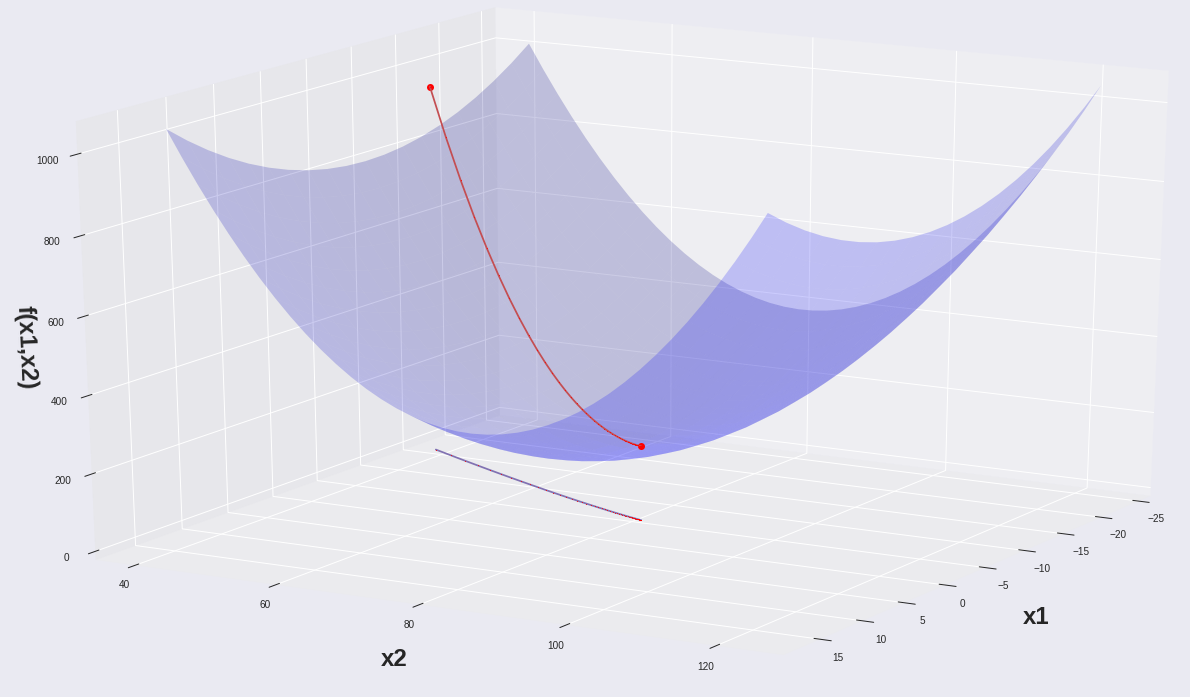
\includegraphics[width=1.0\linewidth]{images/Minimization_image.png}
\end{figure}

\end{frame}

\begin{frame}[fragile]{Descida do gradiente}
\Large{
Na tarefa de aprendizado temos:

\begin{equation*}
J(\vect{\theta}) = \frac{1}{N}\sum_{i=1}^{N} L(\vect{y}^{(i)}, {\hat{\vect{y}}}^{(i)})
\end{equation*}

\begin{equation*}
\vect{\theta}^{novo} = \vect{\theta}^{velho} - \alpha \grad{\vect{\theta}}{J(\vect{\theta})}
\end{equation*}
}
\end{frame}

\begin{frame}[fragile]{Descida do gradiente estocástica}
Na prática nunca lidamos com todos os dados pois $N$ pode ser muito grande (por exemplo, $60$k).\\

Uma alternativa é o algoritmo de \textbf{descida do gradiente estocástica} (\alert{stochastic gradient descent}):

\begin{itemize}
\item Escolhemos uma observação arbitrária $(\vect{x}^{(i)},y^{(i)})$.
\vspace{0.3cm}
\item $J(\vect{\theta}) = L(\vect{y}^{(i)}, {\hat{\vect{y}}}^{(i)})$
\vspace{0.3cm}
\item $\vect{\theta}^{novo} = \vect{\theta}^{velho} - \alpha \grad{\vect{\theta}}{J(\vect{\theta})}$
\end{itemize}

\end{frame}

\begin{frame}[fragile]{Descida do gradiente em lote}
Uma variação desse algoritmo é conhecido como \textbf{descida do gradiente em lote} (\alert{mini-batch gradient descent}):

\begin{itemize}
\item Escolhemos um conjunto de $m$ ($m \ll N$) observações arbitrárias $(\vect{x}^{(1)},y^{(1)}), \dots, (\vect{x}^{(m)},y^{(m)})$.
\vspace{0.3cm}
\item $J(\vect{\theta}) =  \frac{1}{m}\sum_{i=1}^{m} L(\vect{y}^{(i)}, {\hat{\vect{y}}}^{(i)})$
\vspace{0.3cm}
\item $\vect{\theta}^{novo} = \vect{\theta}^{velho} - \alpha \grad{\vect{\theta}}{J(\vect{\theta})}$
\end{itemize}
Quando se processa todos (ou um número equivalente de) exemplos se diz que se passou uma \textbf{época} (\alert{epoch}).
\end{frame}

\begin{frame}[fragile]{Regularização}
Estratégias para impor a navalha de Occam. Elas melhoram a performance no teste às custas de uma piora no treino.
\vspace{0.3cm}
\begin{itemize}
	\item Penalizações à Norma do Parâmetro ($L_2, L_1$)\\
    \vspace{0.3cm}
    \item Early Stopping
    \vspace{0.3cm}
    \item Dropout
    
\end{itemize}
\end{frame}

\begin{frame}[fragile]{Dropout}
\begin{figure}[ht!]
\centering

\scalebox{1.3}{
\begin{tikzpicture}[auto]

% operations =============================
\node[op] (x2) {$x_2$};
\node[op, above=20pt of x2] (x1) {$x_1$};
\node[op, below=20pt of x2] (x3) {$x_3$};
\node[op, above right=10pt and 40pt of x2] (h2) {$h_2$};
\node[op, above=20pt of h2] (h1) {$h_1$};
\node[op, below=20pt of h2] (h3) {$h_3$};
\node[op, below=20pt of h3] (h4) {$h_4$};
\node[op, right=90pt of x2] (o) {$\hat{y}$};

% edges
\path[tedge_dashed] (x1) edge node[pos=0.25, above=1.8pt, dashed] {\large{\alert{$0$}}} (h1);
\path[tedge] (x1) edge node[above=1.2pt] {} (h2);
\path[tedge] (x1) edge node[above=1.8pt] {} (h3);
\path[tedge] (x1) edge node[above=1.8pt] {} (h4);

\path[tedge] (x2) edge node[above=1.8pt] {} (h1);
\path[tedge] (x2) edge node[above=1.8pt] {} (h2);
\path[tedge] (x2) edge node[above=1.8pt] {} (h3);
\path[tedge] (x2) edge node[above=1.8pt] {} (h4);

\path[tedge] (x3) edge node[above=1.8pt] {} (h1);
\path[tedge] (x3) edge node[above=1.8pt] {} (h2);
\path[tedge] (x3) edge node[above=1.8pt] {} (h3);
\path[tedge_dashed] (x3) edge node[above=1.0pt] {} (h4);

\path[tedge_dashed] (h1) edge node[pos=0.25, above=1.8pt, right=0.1cm] {} (o);
\path[tedge] (h2) edge node[above=1.8pt] {} (o);
\path[tedge] (h3) edge node[above=1.8pt] {} (o);
\path[tedge] (h4) edge node[above=1.8pt] {} (o);


% info edges


\end{tikzpicture}
} % scalebox
\end{figure}
\end{frame}

\begin{frame}[fragile]{Dropout}
\begin{figure}[ht!]
\centering

\scalebox{1.3}{
\begin{tikzpicture}[auto]

% operations =============================
\node[op] (x2) {$x_2$};
\node[op, above=20pt of x2] (x1) {$x_1$};
\node[op, below=20pt of x2] (x3) {$x_3$};
\node[op, above right=10pt and 40pt of x2] (h2) {$h_2$};
\node[op, above=20pt of h2] (h1) {$h_1$};
\node[op, below=20pt of h2] (h3) {$h_3$};
\node[op, below=20pt of h3] (h4) {$h_4$};
\node[op, right=90pt of x2] (o) {$\hat{y}$};
% edges
\path[tedge] (x1) edge node[pos=0.25, above=1.8pt] {} (h1);
\path[tedge] (x1) edge node[above=1.2pt] {} (h2);
\path[tedge] (x1) edge node[above=1.8pt] {} (h3);
\path[tedge_dashed] (x1) edge node[above=1.8pt] {} (h4);

\path[tedge] (x2) edge node[above=1.8pt] {} (h1);
\path[tedge_dashed] (x2) edge node[above=1.8pt] {} (h2);
\path[tedge] (x2) edge node[above=1.8pt] {} (h3);
\path[tedge] (x2) edge node[above=1.8pt] {} (h4);

\path[tedge_dashed] (x3) edge node[above=1.8pt] {} (h1);
\path[tedge] (x3) edge node[above=1.8pt] {} (h2);
\path[tedge] (x3) edge node[above=1.8pt] {} (h3);
\path[tedge] (x3) edge node[above=1.0pt] {} (h4);

\path[tedge] (h1) edge node[pos=0.25, above=1.8pt, right=0.1cm] {} (o);
\path[tedge] (h2) edge node[above=1.8pt] {} (o);
\path[tedge] (h3) edge node[above=1.8pt] {} (o);
\path[tedge_dashed] (h4) edge node[below=1.8pt] {\large{\alert{$0$}}}(o);


% info edges


\end{tikzpicture}
} % scalebox
\end{figure}

\end{frame}

\section{Back Propagation}

\begin{frame}{Treinando um modelo}
\Large{
\begin{itemize}
\item $\hat{\vect{y}} = f(\vect{x}; \vect{\theta})$ 
\item $J(\vect{\theta}) =  \frac{1}{m}\sum_{i=1}^{m} L(\vect{y}^{(i)}, {\hat{\vect{y}}}^{(i)})$ 
\item \textbf{SGD}:
\begin{equation*}
\vect{\theta}^{novo} = \vect{\theta}^{velho} - \alpha \grad{\vect{\theta}}{J(\vect{\theta})}
\end{equation*}
\vspace{0.3cm}
\visible<2->{\item Retro propagação (back propagation) é um modo de computar $\grad{\vect{\theta}}{J(\vect{\theta})}$ usando aplicações recursivas da \alert{regra da cadeia}.}
\end{itemize}
}

\end{frame}

\begin{frame}{Operações simples: soma}
\begin{figure}[ht!]
\centering

\scalebox{1.2}{
\begin{tikzpicture}[auto]

% operations =============================
\node[op] (times) {$+$};
\node[op, above left=20pt of times] (a) {$a$};
\node[op, below left=20pt of times] (b) {$b$};
\node[gradient, above=15pt of a] (da) {$\frac{\partial f}{\partial a}$};
\node[gradient, below=15pt of b] (db) {$\frac{\partial f}{\partial b}$};
\node[textonly, right=0.1pt of da] {$=1$};
\node[textonly, right=0.1pt of db] {$=1$};
\node[textonly, right=0.1pt of times] {$=f(a,b) = a+b$};

% edges
\path[tedge] (a) -- (times);
\path[tedge] (b) -- (times);
\path[tedge] (a) -- (da);
\path[tedge] (b) -- (db);


\end{tikzpicture}
} % scalebox
\end{figure}

\end{frame}

\begin{frame}{Operações simples: multiplicação}
\begin{figure}[ht!]
\centering

\scalebox{1.2}{
\begin{tikzpicture}[auto]

% operations =============================
\node[op] (times) {$\times$};
\node[op, above left=20pt of times] (a) {$a$};
\node[op, below left=20pt of times] (b) {$b$};
\node[gradient, above=15pt of a] (da) {$\frac{\partial f}{\partial a}$};
\node[gradient, below=15pt of b] (db) {$\frac{\partial f}{\partial b}$};
\node[textonly, right=0.1pt of da] {$=b$};
\node[textonly, right=0.1pt of db] {$=a$};
\node[textonly, right=0.1pt of times] {$=f(a,b) =a*b$};

% edges
\path[tedge] (a) -- (times);
\path[tedge] (b) -- (times);
\path[tedge] (a) -- (da);
\path[tedge] (b) -- (db);


\end{tikzpicture}
} % scalebox
\end{figure}

\end{frame}

\begin{frame}{Operações simples: divisão}
\begin{figure}[ht!]
\centering

\scalebox{1.2}{
\begin{tikzpicture}[auto]

% operations =============================
\node[op] (times) {$div$};
\node[op, above left=20pt of times] (a) {$a$};
\node[op, below left=20pt of times] (b) {$b$};
\node[gradient, above=15pt of a] (da) {$\frac{\partial f}{\partial a}$};
\node[gradient, below=15pt of b] (db) {$\frac{\partial f}{\partial b}$};
\node[textonly, right=0.1pt of da] {$=\frac{1}{b}$};
\node[textonly, right=0.1pt of db] {$=\frac{-a}{b^{2}}$};
\node[textonly, right=0.1pt of times] {$=f(a,b) =\frac{a}{b}$};

% edges
\path[tedge] (a) -- (times);
\path[tedge] (b) -- (times);
\path[tedge] (a) -- (da);
\path[tedge] (b) -- (db);


\end{tikzpicture}
} % scalebox
\end{figure}

\end{frame}

\begin{frame}{Operações simples: negativo}
\begin{figure}[ht!]
\centering

\scalebox{1.5}{
\begin{tikzpicture}[auto]

% operations =============================
\node[op] (times) {$*-1$};
\node[op, left=20pt of times] (a) {$a$};
\node[gradient, above=30pt of a] (da) {$\frac{df}{da}$};
\node[textonly, right=0.1pt of da] {$=-1$};
\node[textonly, right=0.1pt of times] {$=f(a) =-a$};

% edges
\path[tedge] (a) -- (times);
\path[tedge] (a) -- (da);

\end{tikzpicture}
} % scalebox
\end{figure}

\end{frame}

\begin{frame}{Operações simples: exponenciação}
\begin{figure}[ht!]
\centering

\scalebox{1.5}{
\begin{tikzpicture}[auto]

% operations =============================
\node[op] (times) {$exp$};
\node[op, left=20pt of times] (a) {$a$};
\node[gradient, above=30pt of a] (da) {$\frac{df}{da}$};
\node[textonly, right=0.1pt of da] {$=e^{a}$};
\node[textonly, right=0.1pt of times] {$=f(a) = e^{a}$};

% edges
\path[tedge] (a) -- (times);
\path[tedge] (a) -- (da);

\end{tikzpicture}
} % scalebox
\end{figure}

\end{frame}

\begin{frame}{Operações simples: logarítimo}
\begin{figure}[ht!]
\centering

\scalebox{1.5}{
\begin{tikzpicture}[auto]

% operations =============================
\node[op] (times) {$\log$};
\node[op, left=20pt of times] (a) {$a$};
\node[gradient, above=30pt of a] (da) {$\frac{df}{da}$};
\node[textonly, right=0.1pt of da] {$=\frac{1}{a}$};
\node[textonly, right=0.1pt of times] {$=f(a)=\log(a)$};

% edges
\path[tedge] (a) -- (times);
\path[tedge] (a) -- (da);

\end{tikzpicture}
} % scalebox
\end{figure}

\end{frame}

\begin{frame}{Regra da cadeia}
\Large{
\begin{itemize}
\item $f:\mathbb{R} \rightarrow\mathbb{R}$, $g:\mathbb{R} \rightarrow\mathbb{R}$. 
\item $y = g(x)$
\item $z = f(g(x)) = f(y)$
\end{itemize}
\[
\frac{dz}{dx} = \frac{dz}{dy} \frac{dy}{dx} 
\]
}
\end{frame}


\begin{frame}{Aplicando a regra da cadeia}
\begin{figure}[ht!]
\centering

\scalebox{0.8}{
\begin{tikzpicture}[auto]

% operations =============================
\node[op] (nt) {$n_t$};
\node[op, above left=50pt of nt] (a) {$n^{a}_{t-1}$};
\node[op, below left=40pt of nt] (b) {$n^{b}_{t-1}$};
\node[op, right=40pt of nt] (ntp) {$n_{t+1}$};
\node[textonly, right=20pt of ntp] (ntpp) {$\dots$};
\node[gradient, above=15pt of a] (da) {$\frac{\partial n_{t}}{\partial n^{a}_{t-1}}$};
\node[gradient, above=15pt of nt] (dnt) {$\frac{\partial n_{t+1}}{\partial n_{t}}$};
\node[gradient2, above=15pt of ntp] (dntp) {$\frac{\partial L}{\partial n_{t+1}}$};
\node[gradient2, above=15pt of dnt] (ddnt) {$\frac{\partial L}{\partial n_{t}}$};
\node[gradient2, above left=50pt of ddnt] (dda) {$\frac{\partial L}{\partial n^{a}_{t-1}}$};

% edges =============================
\path[tedge] (a) -- (nt);
\path[tedge] (b) -- (nt);
\path[tedge] (nt) -- (ntp);
\path[tedge] (nt) -- (dnt);
\path[tedge] (ntp) -- (ntpp);
\path[tedge] (ntp) -- (dntp);
\path[tedge] (a) -- (da);
\path[tedge] (dnt) -- (ddnt);
\path[tedge] (dntp) -- (ddnt);
\path[tedge] (da) -- (dda);
\path[tedge] (ddnt) -- (dda);


\end{tikzpicture}
} % scalebox
\end{figure}

\end{frame}

\begin{frame}{Regra da cadeia para várias variáveis}
\Large{
\begin{itemize}
\item $z = f(x,y)$
\item $x = f_{1}(a)$. 
\item $y = f_{2}(a)$
\end{itemize}
\[
\frac{\partial z}{ \partial a} = \frac{\partial z}{\partial x} \frac{\partial x}{\partial a} + \frac{\partial z}{\partial y} \frac{\partial y}{\partial a} 
\]
}
\end{frame}


\begin{frame}{Exemplo}
\begin{figure}[ht!]
\centering

\scalebox{1.2}{
\begin{tikzpicture}[auto]

% operations =============================
\node[op] (div) {$div$};
\node[textonly, right=0.1pt of div] {$=f(x,y)=\frac{x}{y}=\frac{a*c}{a+b}$};
\node[op, above left=20pt of div] (mult) {$*$};
\node[op, below left=20pt of div] (plus) {$+$};
\node[op, below=20pt of plus] (b2) {$b$};
\node[op, above=20pt of mult] (b1) {$c$};
\node[op, left=55pt of div] (a) {$a$};
\node[textonly, above right=5pt and 5pt of div] (inv1) {$\frac{\partial f}{\partial x} \frac{\partial x}{\partial a}$};
\node[textonly, above left=2pt and 2pt of a] (inv2) {};
\node[textonly, below right=5pt and 5pt of div] (inv3) {$\frac{\partial f}{\partial y} \frac{\partial y}{\partial a}$};
\node[textonly, below left=2pt and 2pt of a] (inv4) {};


% edges
\path[tedge] (a) -- (mult);
\path[tedge] (b1) -- (mult);
\path[tedge] (a) -- (plus);
\path[tedge] (b2) -- (plus);
\path[tedge] (plus) -- (div);
\path[tedge] (mult) -- (div);
\path[tedge, nephritis!60, line width=1mm] (inv1) to [out=120,in=80] (inv2);
\path[tedge, nephritis!60, line width=1mm] (inv3) to [out=-120,in=-80] (inv4);



\end{tikzpicture}
} % scalebox
\end{figure}

\end{frame}

\begin{frame}{Exemplo: regressão logística}
\Large{
\begin{equation*}
\hat{\vect{y}} = softmax(\vect{W}\vect{x} + \vect{b})
\end{equation*}
\begin{equation*}
L(\vect{y},\hat{\vect{y}}) = CE(\vect{y},\hat{\vect{y}})
\end{equation*}


\begin{equation*}
L(\vect{y},\hat{\vect{y}}) = - \sum_{i}\vect{y}_{i} \log \left(\frac{exp(\sum_{k} \vect{W}_{i,k}\vect{x}_{k} + \vect{b}_{i})}{\sum_{j}exp(\sum_{k}\vect{W}_{j,k}\vect{x}_{k} + \vect{b}_{j})} \right)
\end{equation*}
}
\end{frame}

\begin{frame}{Simplificação}
\Large{
\begin{itemize}
\item $\begin{bmatrix}z_1\\z_2\end{bmatrix} = \begin{bmatrix}w_{11}  & w_{12}\\w_{21}  & w_{22}\end{bmatrix}* \begin{bmatrix}x_1\\x_2\end{bmatrix} + \begin{bmatrix}b_1\\b_2\end{bmatrix}$

\vspace{0.4cm}

\item $\begin{bmatrix}h_1\\h_2\end{bmatrix} = \begin{bmatrix}exp(z_1)\\exp(z_2)\end{bmatrix}$ 

\vspace{0.4cm}

\item $H = h_1 + h_2$ 

\vspace{0.4cm}

\item $\begin{bmatrix}\hat{y}_1\\\hat{y}_2\end{bmatrix} = \begin{bmatrix}\frac{h_1}{H}\\\frac{h_2}{H}\end{bmatrix}$ 
\end{itemize}
}
\end{frame}



\begin{frame}{Grafo de $L(\hat{\vect{y}}, \vect{y})$}
\begin{figure}[ht!]
\centering

\scalebox{0.6}{
\begin{tikzpicture}[auto]

% operations =============================

% input x and W
\node[op] (w11) {$w_{11}$};
\node[placeholder, below=10pt of w11] (x1) {$x_{1}$};
\node[op, below=20pt of x1] (w12) {$w_{12}$};
\node[placeholder, below=10pt of w12] (x2) {$x_{2}$};

\node[op, below=20pt of x2] (w21) {$w_{21}$};
\node[placeholder, below=10pt of w21] (x11) {$x_{1}$};
\node[op, below=20pt of x11] (w22) {$w_{22}$};
\node[placeholder, below=10pt of w22] (x22) {$x_{2}$};

% multiplication
\node[op, below right=1pt and 20pt of w11] (mult1) {$*$};
\node[op, below right=1pt and 20pt of w12] (mult2) {$*$};
\node[op, below right=1pt and 20pt of w21] (mult3) {$*$};
\node[op, below right=1pt and 20pt of w22] (mult4) {$*$};

% sum
\node[op, below right=25pt and 20pt of mult1] (sum1) {$+$};
\node[op, below right=25pt and 20pt of mult3] (sum2) {$+$};
\node[op, right=25pt of sum1] (sum3) {$z_1$};
\node[op, right=25pt of sum2] (sum4) {$z_2$};
\node[op, above left=25pt and 10pt of sum3] (b1) {$b_1$};
\node[op, below left=25pt and 10pt of sum4] (b2) {$b_2$};

% exp
\node[op, right=25pt of sum3] (exp1) {$h_1$};
\node[op, right=25pt of sum4] (exp2) {$h_2$};
\node[op, below right=65pt and 15pt of exp1] (sum5) {$H$};
\node[op, right=35pt of exp1] (div1) {$\hat{y}_1$};
\node[op, right=35pt of exp2] (div2) {$\hat{y}_2$};

% log
\node[op, right=25pt of div1] (log1) {$\log$};
\node[op, right=25pt of div2] (log2) {$\log$};
\node[op, right=25pt of log1] (mult5) {$*$};
\node[op, right=25pt of log2] (mult6) {$*$};
\node[placeholder, above left=25pt and 10pt of mult5] (y1) {$y_1$};
\node[placeholder, below left=25pt and 10pt of mult6] (y2) {$y_2$};
\node[op, below right=65pt and 15pt of mult5] (sum6) {$+$};
\node[op, right=25pt of sum6] (minus1) {$*-1$};



%edges
\path[tedge] (w11) -- (mult1);
\path[tedge] (x1) -- (mult1);
\path[tedge] (w12) -- (mult2);
\path[tedge] (x2) -- (mult2);
\path[tedge] (w21) -- (mult3);
\path[tedge] (x11) -- (mult3);
\path[tedge] (w22) -- (mult4);
\path[tedge] (x22) -- (mult4);

\path[tedge] (mult1) -- (sum1);
\path[tedge] (mult2) -- (sum1);
\path[tedge] (mult3) -- (sum2);
\path[tedge] (mult4) -- (sum2);
\path[tedge] (sum1) -- (sum3);
\path[tedge] (b1) -- (sum3);
\path[tedge] (sum2) -- (sum4);
\path[tedge] (b2) -- (sum4);

\path[tedge] (sum3) -- (exp1);
\path[tedge] (sum4) -- (exp2);
\path[tedge] (exp1) -- (sum5);
\path[tedge] (exp2) -- (sum5);
\path[tedge] (exp1) -- (div1);
\path[tedge] (exp2) -- (div2);
\path[tedge] (sum5) -- (div1);
\path[tedge] (sum5) -- (div2);


\path[tedge] (div1) -- (log1);
\path[tedge] (div2) -- (log2);
\path[tedge] (log1) -- (mult5);
\path[tedge] (y1) -- (mult5);
\path[tedge] (log2) -- (mult6);
\path[tedge] (y2) -- (mult6);
\path[tedge] (mult5) -- (sum6);
\path[tedge] (mult6) -- (sum6);
\path[tedge] (sum6) -- (minus1);

\end{tikzpicture}
} % scalebox
\end{figure}

\end{frame}

\begin{frame}{Caminho de $b_1$: 1}
\begin{figure}[ht!]
\centering

\scalebox{0.6}{
\begin{tikzpicture}[auto]

% operations =============================

% input x and W
\node[op] (w11) {$w_{11}$};
\node[op, below=10pt of w11] (x1) {$x_{1}$};
\node[op, below=20pt of x1] (w12) {$w_{12}$};
\node[op, below=10pt of w12] (x2) {$x_{2}$};

\node[op, below=20pt of x2] (w21) {$w_{21}$};
\node[op, below=10pt of w21] (x11) {$x_{1}$};
\node[op, below=20pt of x11] (w22) {$w_{22}$};
\node[op, below=10pt of w22] (x22) {$x_{2}$};

% multiplication
\node[op, below right=1pt and 20pt of w11] (mult1) {$*$};
\node[op, below right=1pt and 20pt of w12] (mult2) {$*$};
\node[op, below right=1pt and 20pt of w21] (mult3) {$*$};
\node[op, below right=1pt and 20pt of w22] (mult4) {$*$};

% sum
\node[op, below right=25pt and 20pt of mult1] (sum1) {$+$};
\node[op, below right=25pt and 20pt of mult3] (sum2) {$+$};
\node[op2, right=25pt of sum1] (sum3) {$z_1$};
\node[op, right=25pt of sum2] (sum4) {$z_2$};
\node[op2, above left=25pt and 10pt of sum3] (b1) {$b_1$};
\node[op, below left=25pt and 10pt of sum4] (b2) {$b_2$};

% exp
\node[op2, right=25pt of sum3] (exp1) {$h_1$};
\node[op, right=25pt of sum4] (exp2) {$h_2$};
\node[op, below right=65pt and 15pt of exp1] (sum5) {$H$};
\node[op2, right=35pt of exp1] (div1) {$\hat{y}_1$};
\node[op, right=35pt of exp2] (div2) {$\hat{y}_2$};

% log
\node[op2, right=25pt of div1] (log1) {$\log$};
\node[op, right=25pt of div2] (log2) {$\log$};
\node[op2, right=25pt of log1] (mult5) {$*$};
\node[op, right=25pt of log2] (mult6) {$*$};
\node[op, above left=25pt and 10pt of mult5] (y1) {$y_1$};
\node[op, below left=25pt and 10pt of mult6] (y2) {$y_2$};
\node[op2, below right=65pt and 15pt of mult5] (sum6) {$+$};
\node[op2, right=25pt of sum6] (minus1) {$*-1$};



%edges
\path[tedge] (w11) -- (mult1);
\path[tedge] (x1) -- (mult1);
\path[tedge] (w12) -- (mult2);
\path[tedge] (x2) -- (mult2);
\path[tedge] (w21) -- (mult3);
\path[tedge] (x11) -- (mult3);
\path[tedge] (w22) -- (mult4);
\path[tedge] (x22) -- (mult4);

\path[tedge] (mult1) -- (sum1);
\path[tedge] (mult2) -- (sum1);
\path[tedge] (mult3) -- (sum2);
\path[tedge] (mult4) -- (sum2);
\path[tedge] (sum1) -- (sum3);
\path[tedge] (b1) -- (sum3);
\path[tedge] (sum2) -- (sum4);
\path[tedge] (b2) -- (sum4);

\path[tedge] (sum3) -- (exp1);
\path[tedge] (sum4) -- (exp2);
\path[tedge] (exp1) -- (sum5);
\path[tedge] (exp2) -- (sum5);
\path[tedge] (exp1) -- (div1);
\path[tedge] (exp2) -- (div2);
\path[tedge] (sum5) -- (div1);
\path[tedge] (sum5) -- (div2);


\path[tedge] (div1) -- (log1);
\path[tedge] (div2) -- (log2);
\path[tedge] (log1) -- (mult5);
\path[tedge] (y1) -- (mult5);
\path[tedge] (log2) -- (mult6);
\path[tedge] (y2) -- (mult6);
\path[tedge] (mult5) -- (sum6);
\path[tedge] (mult6) -- (sum6);
\path[tedge] (sum6) -- (minus1);

\end{tikzpicture}
} % scalebox
\end{figure}

\end{frame}

\begin{frame}{Caminho de $b_1$: 2}
\begin{figure}[ht!]
\centering

\scalebox{0.6}{
\begin{tikzpicture}[auto]

% operations =============================

% input x and W
\node[op] (w11) {$w_{11}$};
\node[op, below=10pt of w11] (x1) {$x_{1}$};
\node[op, below=20pt of x1] (w12) {$w_{12}$};
\node[op, below=10pt of w12] (x2) {$x_{2}$};

\node[op, below=20pt of x2] (w21) {$w_{21}$};
\node[op, below=10pt of w21] (x11) {$x_{1}$};
\node[op, below=20pt of x11] (w22) {$w_{22}$};
\node[op, below=10pt of w22] (x22) {$x_{2}$};

% multiplication
\node[op, below right=1pt and 20pt of w11] (mult1) {$*$};
\node[op, below right=1pt and 20pt of w12] (mult2) {$*$};
\node[op, below right=1pt and 20pt of w21] (mult3) {$*$};
\node[op, below right=1pt and 20pt of w22] (mult4) {$*$};

% sum
\node[op, below right=25pt and 20pt of mult1] (sum1) {$+$};
\node[op, below right=25pt and 20pt of mult3] (sum2) {$+$};
\node[op2, right=25pt of sum1] (sum3) {$z_1$};
\node[op, right=25pt of sum2] (sum4) {$z_2$};
\node[op2, above left=25pt and 10pt of sum3] (b1) {$b_1$};
\node[op, below left=25pt and 10pt of sum4] (b2) {$b_2$};

% exp
\node[op2, right=25pt of sum3] (exp1) {$h_1$};
\node[op, right=25pt of sum4] (exp2) {$h_2$};
\node[op2, below right=65pt and 15pt of exp1] (sum5) {$H$};
\node[op2, right=35pt of exp1] (div1) {$\hat{y}_1$};
\node[op, right=35pt of exp2] (div2) {$\hat{y}_2$};

% log
\node[op2, right=25pt of div1] (log1) {$\log$};
\node[op, right=25pt of div2] (log2) {$\log$};
\node[op2, right=25pt of log1] (mult5) {$*$};
\node[op, right=25pt of log2] (mult6) {$*$};
\node[op, above left=25pt and 10pt of mult5] (y1) {$y_1$};
\node[op, below left=25pt and 10pt of mult6] (y2) {$y_2$};
\node[op2, below right=65pt and 15pt of mult5] (sum6) {$+$};
\node[op2, right=25pt of sum6] (minus1) {$*-1$};



%edges
\path[tedge] (w11) -- (mult1);
\path[tedge] (x1) -- (mult1);
\path[tedge] (w12) -- (mult2);
\path[tedge] (x2) -- (mult2);
\path[tedge] (w21) -- (mult3);
\path[tedge] (x11) -- (mult3);
\path[tedge] (w22) -- (mult4);
\path[tedge] (x22) -- (mult4);

\path[tedge] (mult1) -- (sum1);
\path[tedge] (mult2) -- (sum1);
\path[tedge] (mult3) -- (sum2);
\path[tedge] (mult4) -- (sum2);
\path[tedge] (sum1) -- (sum3);
\path[tedge] (b1) -- (sum3);
\path[tedge] (sum2) -- (sum4);
\path[tedge] (b2) -- (sum4);

\path[tedge] (sum3) -- (exp1);
\path[tedge] (sum4) -- (exp2);
\path[tedge] (exp1) -- (sum5);
\path[tedge] (exp2) -- (sum5);
\path[tedge] (exp1) -- (div1);
\path[tedge] (exp2) -- (div2);
\path[tedge] (sum5) -- (div1);
\path[tedge] (sum5) -- (div2);


\path[tedge] (div1) -- (log1);
\path[tedge] (div2) -- (log2);
\path[tedge] (log1) -- (mult5);
\path[tedge] (y1) -- (mult5);
\path[tedge] (log2) -- (mult6);
\path[tedge] (y2) -- (mult6);
\path[tedge] (mult5) -- (sum6);
\path[tedge] (mult6) -- (sum6);
\path[tedge] (sum6) -- (minus1);

\end{tikzpicture}
} % scalebox
\end{figure}

\end{frame}

\begin{frame}{Caminho de $b_1$: 3}
\begin{figure}[ht!]
\centering

\scalebox{0.6}{
\begin{tikzpicture}[auto]

% operations =============================

% input x and W
\node[op] (w11) {$w_{11}$};
\node[op, below=10pt of w11] (x1) {$x_{1}$};
\node[op, below=20pt of x1] (w12) {$w_{12}$};
\node[op, below=10pt of w12] (x2) {$x_{2}$};

\node[op, below=20pt of x2] (w21) {$w_{21}$};
\node[op, below=10pt of w21] (x11) {$x_{1}$};
\node[op, below=20pt of x11] (w22) {$w_{22}$};
\node[op, below=10pt of w22] (x22) {$x_{2}$};

% multiplication
\node[op, below right=1pt and 20pt of w11] (mult1) {$*$};
\node[op, below right=1pt and 20pt of w12] (mult2) {$*$};
\node[op, below right=1pt and 20pt of w21] (mult3) {$*$};
\node[op, below right=1pt and 20pt of w22] (mult4) {$*$};

% sum
\node[op, below right=25pt and 20pt of mult1] (sum1) {$+$};
\node[op, below right=25pt and 20pt of mult3] (sum2) {$+$};
\node[op2, right=25pt of sum1] (sum3) {$z_1$};
\node[op, right=25pt of sum2] (sum4) {$z_2$};
\node[op2, above left=25pt and 10pt of sum3] (b1) {$b_1$};
\node[op, below left=25pt and 10pt of sum4] (b2) {$b_2$};

% exp
\node[op2, right=25pt of sum3] (exp1) {$h_1$};
\node[op, right=25pt of sum4] (exp2) {$h_2$};
\node[op2, below right=65pt and 15pt of exp1] (sum5) {$H$};
\node[op, right=35pt of exp1] (div1) {$\hat{y}_1$};
\node[op2, right=35pt of exp2] (div2) {$\hat{y}_2$};

% log
\node[op, right=25pt of div1] (log1) {$\log$};
\node[op2, right=25pt of div2] (log2) {$\log$};
\node[op, right=25pt of log1] (mult5) {$*$};
\node[op2, right=25pt of log2] (mult6) {$*$};
\node[op, above left=25pt and 10pt of mult5] (y1) {$y_1$};
\node[op, below left=25pt and 10pt of mult6] (y2) {$y_2$};
\node[op2, below right=65pt and 15pt of mult5] (sum6) {$+$};
\node[op2, right=25pt of sum6] (minus1) {$*-1$};



%edges
\path[tedge] (w11) -- (mult1);
\path[tedge] (x1) -- (mult1);
\path[tedge] (w12) -- (mult2);
\path[tedge] (x2) -- (mult2);
\path[tedge] (w21) -- (mult3);
\path[tedge] (x11) -- (mult3);
\path[tedge] (w22) -- (mult4);
\path[tedge] (x22) -- (mult4);

\path[tedge] (mult1) -- (sum1);
\path[tedge] (mult2) -- (sum1);
\path[tedge] (mult3) -- (sum2);
\path[tedge] (mult4) -- (sum2);
\path[tedge] (sum1) -- (sum3);
\path[tedge] (b1) -- (sum3);
\path[tedge] (sum2) -- (sum4);
\path[tedge] (b2) -- (sum4);

\path[tedge] (sum3) -- (exp1);
\path[tedge] (sum4) -- (exp2);
\path[tedge] (exp1) -- (sum5);
\path[tedge] (exp2) -- (sum5);
\path[tedge] (exp1) -- (div1);
\path[tedge] (exp2) -- (div2);
\path[tedge] (sum5) -- (div1);
\path[tedge] (sum5) -- (div2);


\path[tedge] (div1) -- (log1);
\path[tedge] (div2) -- (log2);
\path[tedge] (log1) -- (mult5);
\path[tedge] (y1) -- (mult5);
\path[tedge] (log2) -- (mult6);
\path[tedge] (y2) -- (mult6);
\path[tedge] (mult5) -- (sum6);
\path[tedge] (mult6) -- (sum6);
\path[tedge] (sum6) -- (minus1);

\end{tikzpicture}
} % scalebox
\end{figure}

\end{frame}

\begin{frame}{Derivada parcial de L com respeito a $b_1$: 1}
\begin{figure}[ht!]
\centering

\scalebox{0.8}{
\begin{tikzpicture}[auto]

% operations =============================

% multiplication
\node[op] (z1) {$z_1$};
\node[op, above left=25pt and 20pt of z1] (b1) {$b_1$};

% exp
\node[op, right=25pt of z1] (exp1) {$h_1$};
\node[op, right=35pt of exp1] (div1) {$\hat{y}_1$};
\node[op, below left=25pt and 10pt of div1] (H) {$H$};

% log
\node[op, right=25pt of div1] (log1) {$\log$};
\node[op, right=25pt of log1] (mult5) {$*$};
\node[op, right=25pt of mult5] (sum6) {$+$};
\node[op, right=25pt of sum6] (minus1) {$*-1$};
\node[op, below left=25pt and 10pt of mult5] (y1) {$y_1$};
\node[textonly, below left=55pt and 10pt of sum6] (dots) {{\LARGE$\dots$}};

%gradients 1
\node[gradient, above=10pt of sum6] (dsum6) {$-1$};
\node[gradient, above=10pt of mult5] (dmult5) {$1$};
\node[gradient, above=10pt of log1] (dlog1) {$y_1$};
\node[gradient, above=10pt of div1] (ddiv1) {$\frac{H}{h_1}$};
\node[gradient, above=10pt of exp1] (dexp1) {$\frac{1}{H}$};
\node[gradient, above=10pt of z1] (dz1) {$h_1$};
\node[gradient, above=10pt of b1] (db1) {$1$};

%gradients 2
\node[gradient2, above left=30pt and 10pt of dsum6] (dLdmult5) {$-1$};
\node[gradient2, left=25pt of dLdmult5] (dLlog1) {$-y_1$};
\node[gradient2, left=25pt of dLlog1] (dLdiv1) {$-y_1\frac{H}{h_1}$};
\node[gradient2, left=25pt of dLdiv1] (dLdexp1) {$\frac{-y_1}{h_1}$};
\node[gradient2, left=25pt of dLdexp1] (dLdz1) {$-y_1$};
\node[gradient2, above=35pt of db1] (dLdb1) {$-y_1$};

%edges
\path[tedge] (b1) -- (z1);
\path[tedge] (z1) -- (exp1);
\path[tedge] (exp1) -- (div1);
\path[tedge] (H) -- (div1);
\path[tedge] (div1) -- (log1);
\path[tedge] (log1) -- (mult5);
\path[tedge] (y1) -- (mult5);
\path[tedge] (mult5) -- (sum6);
\path[tedge] (dots) -- (sum6);
\path[tedge] (sum6) -- (minus1);

%edges gradient 1
\path[tedge] (b1) -- (db1);
\path[tedge] (z1) -- (dz1);
\path[tedge] (exp1) -- (dexp1);
\path[tedge] (div1) -- (ddiv1);
\path[tedge] (log1) -- (dlog1);
\path[tedge] (mult5) -- (dmult5);
\path[tedge] (sum6) -- (dsum6);

%edges gradient 2
\path[tedge] (dsum6) -- (dLdmult5);
\path[tedge] (dmult5) -- (dLdmult5);
\path[tedge] (dLdmult5) -- (dLlog1);
\path[tedge] (dlog1) -- (dLlog1);
\path[tedge] (ddiv1) -- (dLdiv1);
\path[tedge] (dLlog1) -- (dLdiv1);
\path[tedge] (dexp1) -- (dLdexp1);
\path[tedge] (dLdiv1) -- (dLdexp1);
\path[tedge] (dz1) -- (dLdz1);
\path[tedge] (dLdexp1) -- (dLdz1);
\path[tedge] (db1) -- (dLdb1);
\path[tedge] (dLdz1) -- (dLdb1);


\end{tikzpicture}
} % scalebox
\end{figure}

\end{frame}

\begin{frame}{Derivada parcial de L com respeito a $b_1$: 2}
\begin{figure}[ht!]
\centering

\scalebox{0.7}{
\begin{tikzpicture}[auto]

% operations =============================

% multiplication
\node[op] (z1) {$z_1$};
\node[op, above left=25pt and 20pt of z1] (b1) {$b_1$};

% exp
\node[op, right=25pt of z1] (exp1) {$h_1$};
\node[op, right=25pt of exp1] (H) {$H$};
\node[op, right=35pt of H] (div1) {$\hat{y}_1$};

% log
\node[op, right=25pt of div1] (log1) {$\log$};
\node[op, right=25pt of log1] (mult5) {$*$};
\node[op, below left=25pt and 10pt of mult5] (y1) {$y_1$};
\node[op, right=25pt of mult5] (sum6) {$+$};
\node[op, right=25pt of sum6] (minus1) {$*-1$};
\node[textonly, below left=55pt and 10pt of sum6] (dots) {{\LARGE$\dots$}};

%gradients 1
\node[gradient, above=10pt of sum6] (dsum6) {$-1$};
\node[gradient, above=10pt of mult5] (dmult5) {$1$};
\node[gradient, above=10pt of log1] (dlog1) {$y_1$};
\node[gradient, above=10pt of div1] (ddiv1) {$\frac{H}{h_1}$};
\node[gradient, above=10pt of H] (dH) {$-\frac{h_1}{H^2}$};
\node[gradient, above=10pt of exp1] (dexp1) {$1$};
\node[gradient, above=10pt of z1] (dz1) {$h_1$};
\node[gradient, above=10pt of b1] (db1) {$1$};

%gradients 2
\node[gradient2, above left=30pt and 10pt of dsum6] (dLdmult5) {$-1$};
\node[gradient2, left=25pt of dLdmult5] (dLlog1) {$-y_1$};
\node[gradient2, left=25pt of dLlog1] (dLdiv1) {$-y_1\frac{H}{h_1}$};
\node[gradient2, left=25pt of dLdiv1] (dLdH) {$\frac{y_1}{H}$};
\node[gradient2, left=25pt of dLdH] (dLdexp1) {$\frac{y_1}{H}$};
\node[gradient2, left=25pt of dLdexp1] (dLdz1) {$y_1\frac{h_1}{H}$};
\node[gradient2, above=35pt of db1] (dLdb1) {$y_1\frac{h_1}{H}$};

%edges
\path[tedge] (b1) -- (z1);
\path[tedge] (z1) -- (exp1);
\path[tedge] (exp1) -- (H);
\path[tedge] (H) -- (div1);

\path[tedge] (div1) -- (log1);
\path[tedge] (log1) -- (mult5);
\path[tedge] (y1) -- (mult5);
\path[tedge] (mult5) -- (sum6);
\path[tedge] (dots) -- (sum6);
\path[tedge] (sum6) -- (minus1);

%edges gradient 1
\path[tedge] (b1) -- (db1);
\path[tedge] (z1) -- (dz1);
\path[tedge] (exp1) -- (dexp1);
\path[tedge] (div1) -- (ddiv1);
\path[tedge] (H) -- (dH);
\path[tedge] (log1) -- (dlog1);
\path[tedge] (mult5) -- (dmult5);
\path[tedge] (sum6) -- (dsum6);

%edges gradient 2
\path[tedge] (dsum6) -- (dLdmult5);
\path[tedge] (dmult5) -- (dLdmult5);
\path[tedge] (dLdmult5) -- (dLlog1);
\path[tedge] (dlog1) -- (dLlog1);
\path[tedge] (ddiv1) -- (dLdiv1);
\path[tedge] (dLlog1) -- (dLdiv1);
\path[tedge] (dexp1) -- (dLdexp1);
\path[tedge] (dH) -- (dLdH);
\path[tedge] (dLdiv1) -- (dLdH);
\path[tedge] (dLdH) -- (dLdexp1);
\path[tedge] (dz1) -- (dLdz1);
\path[tedge] (dLdexp1) -- (dLdz1);
\path[tedge] (db1) -- (dLdb1);
\path[tedge] (dLdz1) -- (dLdb1);


\end{tikzpicture}
} % scalebox
\end{figure}

\end{frame}

\begin{frame}{Derivada parcial de L com respeito a $b_1$: 3}
\begin{figure}[ht!]
\centering

\scalebox{0.7}{
\begin{tikzpicture}[auto]

% operations =============================

% multiplication
\node[op] (z1) {$z_1$};
\node[op, above left=25pt and 20pt of z1] (b1) {$b_1$};

% exp
\node[op, right=25pt of z1] (exp1) {$h_1$};
\node[op, right=25pt of exp1] (H) {$H$};
\node[op, right=35pt of H] (div1) {$\hat{y}_2$};

% log
\node[op, right=25pt of div1] (log1) {$\log$};
\node[op, right=25pt of log1] (mult5) {$*$};
\node[placeholder, below left=25pt and 10pt of mult5] (y2) {$y_2$};
\node[op, right=25pt of mult5] (sum6) {$+$};
\node[op, right=25pt of sum6] (minus1) {$*-1$};
\node[textonly, below left=55pt and 10pt of sum6] (dots) {{\LARGE$\dots$}};

%gradients 1
\node[gradient, above=10pt of sum6] (dsum6) {$-1$};
\node[gradient, above=10pt of mult5] (dmult5) {$1$};
\node[gradient, above=10pt of log1] (dlog1) {$y_2$};
\node[gradient, above=10pt of div1] (ddiv1) {$\frac{H}{h_1}$};
\node[gradient, above=10pt of H] (dH) {$-\frac{h_1}{H^2}$};
\node[gradient, above=10pt of exp1] (dexp1) {$1$};
\node[gradient, above=10pt of z1] (dz1) {$h_1$};
\node[gradient, above=10pt of b1] (db1) {$1$};

%gradients 2
\node[gradient2, above left=30pt and 10pt of dsum6] (dLdmult5) {$-1$};
\node[gradient2, left=25pt of dLdmult5] (dLlog1) {$-y_2$};
\node[gradient2, left=25pt of dLlog1] (dLdiv1) {$-y_2\frac{H}{h_1}$};
\node[gradient2, left=25pt of dLdiv1] (dLdH) {$\frac{y_2}{H}$};
\node[gradient2, left=25pt of dLdH] (dLdexp1) {$\frac{y_2}{H}$};
\node[gradient2, left=25pt of dLdexp1] (dLdz1) {$y_2\frac{h_1}{H}$};
\node[gradient2, above=35pt of db1] (dLdb1) {$y_2\frac{h_1}{H}$};

%edges
\path[tedge] (b1) -- (z1);
\path[tedge] (z1) -- (exp1);
\path[tedge] (exp1) -- (H);
\path[tedge] (H) -- (div1);

\path[tedge] (div1) -- (log1);
\path[tedge] (log1) -- (mult5);
\path[tedge] (y2) -- (mult5);
\path[tedge] (mult5) -- (sum6);
\path[tedge] (dots) -- (sum6);
\path[tedge] (sum6) -- (minus1);

%edges gradient 1
\path[tedge] (b1) -- (db1);
\path[tedge] (z1) -- (dz1);
\path[tedge] (exp1) -- (dexp1);
\path[tedge] (div1) -- (ddiv1);
\path[tedge] (H) -- (dH);
\path[tedge] (log1) -- (dlog1);
\path[tedge] (mult5) -- (dmult5);
\path[tedge] (sum6) -- (dsum6);

%edges gradient 2
\path[tedge] (dsum6) -- (dLdmult5);
\path[tedge] (dmult5) -- (dLdmult5);
\path[tedge] (dLdmult5) -- (dLlog1);
\path[tedge] (dlog1) -- (dLlog1);
\path[tedge] (ddiv1) -- (dLdiv1);
\path[tedge] (dLlog1) -- (dLdiv1);
\path[tedge] (dexp1) -- (dLdexp1);
\path[tedge] (dH) -- (dLdH);
\path[tedge] (dLdiv1) -- (dLdH);
\path[tedge] (dLdH) -- (dLdexp1);
\path[tedge] (dz1) -- (dLdz1);
\path[tedge] (dLdexp1) -- (dLdz1);
\path[tedge] (db1) -- (dLdb1);
\path[tedge] (dLdz1) -- (dLdb1);


\end{tikzpicture}
} % scalebox
\end{figure}

\end{frame}

\begin{frame}{Derivada parcial de L com respeito a $b_1$}
\Large{
\begin{align*}
\frac{\partial L}{\partial b_1} &= -y_1 + y_1\frac{h_1}{H} + y_2\frac{h_1}{H}\\
\vspace{0.2cm}
\visible<2->{&= y_1\left(\frac{h_1}{H} -1\right) + y_2\left(\frac{h_1}{H} -0\right)\\}
\visible<3->{&= y_1\left(\hat{y}_1 -1\right) + y_2\left(\hat{y}_1 -0\right)\\}
\visible<4->{&= \hat{y}_1 - y_1 \;\;\;\; \text{(quando} \;\; y \;\; \text{é um vetor one-hot)}}
\end{align*}
}
\end{frame}

\begin{frame}{Exemplo}
\begin{figure}[ht!]
\centering

\scalebox{1.3}{
\begin{tikzpicture}[auto]

% operations =============================

% nodes
\node[textonly] (W) {$\begin{bmatrix}0.65  & 1.19\\0.69  & -0.92\end{bmatrix}$};
\node[textonly, right=40pt of W] (x) {$\begin{bmatrix}0.2\\0.7\end{bmatrix}$};
\node[textonly, below=30pt of W] (b) {$\begin{bmatrix}0\\0\end{bmatrix}$};
\node[textonly, below=30pt of x] (y) {$\begin{bmatrix}1\\0\end{bmatrix}$};
\node[textonly, left=1pt of W] (Wname) {$\vect{W}=$};
\node[textonly, left=1pt of x] (xname) {$\vect{x}=$};
\node[textonly, left=1pt of b] (bname) {$\vect{b}=$};
\node[textonly, left=1pt of y] (yname) {$\vect{y}=$};


\end{tikzpicture}
} % scalebox
\end{figure}

\end{frame}

\begin{frame}{Forward}
\begin{figure}[ht!]
\centering

\scalebox{0.6}{
\begin{tikzpicture}[auto]

% operations =============================

% input x and W
\node[op] (w11) {$w_{11}$};
\node[placeholder, below=10pt of w11] (x1) {$x_{1}$};
\node[op, below=20pt of x1] (w12) {$w_{12}$};
\node[placeholder, below=10pt of w12] (x2) {$x_{2}$};

\node[op, below=20pt of x2] (w21) {$w_{21}$};
\node[placeholder, below=10pt of w21] (x11) {$x_{1}$};
\node[op, below=20pt of x11] (w22) {$w_{22}$};
\node[placeholder, below=10pt of w22] (x22) {$x_{2}$};

% multiplication
\node[op, below right=1pt and 20pt of w11] (mult1) {$*$};
\node[op, below right=1pt and 20pt of w12] (mult2) {$*$};
\node[op, below right=1pt and 20pt of w21] (mult3) {$*$};
\node[op, below right=1pt and 20pt of w22] (mult4) {$*$};

% sum
\node[op, below right=25pt and 20pt of mult1] (sum1) {$+$};
\node[op, below right=25pt and 20pt of mult3] (sum2) {$+$};
\node[op, right=25pt of sum1] (sum3) {$z_1$};
\node[op, right=25pt of sum2] (sum4) {$z_2$};
\node[op, above left=25pt and 10pt of sum3] (b1) {$b_1$};
\node[op, below left=25pt and 10pt of sum4] (b2) {$b_2$};

% exp
\node[op, right=25pt of sum3] (exp1) {$h_1$};
\node[op, right=25pt of sum4] (exp2) {$h_2$};
\node[op, below right=65pt and 15pt of exp1] (sum5) {$H$};
\node[op, right=35pt of exp1] (div1) {$\hat{y}_1$};
\node[op, right=35pt of exp2] (div2) {$\hat{y}_2$};

% log
\node[op, right=25pt of div1] (log1) {$\log$};
\node[op, right=25pt of div2] (log2) {$\log$};
\node[op, right=25pt of log1] (mult5) {$*$};
\node[op, right=25pt of log2] (mult6) {$*$};
\node[placeholder, above left=25pt and 10pt of mult5] (y1) {$y_1$};
\node[placeholder, below left=25pt and 10pt of mult6] (y2) {$y_2$};
\node[op, below right=65pt and 15pt of mult5] (sum6) {$+$};
\node[op, right=25pt of sum6] (minus1) {$*-1$};



%edges
\path[tedge] (w11) -- (mult1);
\path[tedge] (x1) -- (mult1);
\path[tedge] (w12) -- (mult2);
\path[tedge] (x2) -- (mult2);
\path[tedge] (w21) -- (mult3);
\path[tedge] (x11) -- (mult3);
\path[tedge] (w22) -- (mult4);
\path[tedge] (x22) -- (mult4);

\path[tedge] (mult1) -- (sum1);
\path[tedge] (mult2) -- (sum1);
\path[tedge] (mult3) -- (sum2);
\path[tedge] (mult4) -- (sum2);
\path[tedge] (sum1) -- (sum3);
\path[tedge] (b1) -- (sum3);
\path[tedge] (sum2) -- (sum4);
\path[tedge] (b2) -- (sum4);

\path[tedge] (sum3) -- (exp1);
\path[tedge] (sum4) -- (exp2);
\path[tedge] (exp1) -- (sum5);
\path[tedge] (exp2) -- (sum5);
\path[tedge] (exp1) -- (div1);
\path[tedge] (exp2) -- (div2);
\path[tedge] (sum5) -- (div1);
\path[tedge] (sum5) -- (div2);


\path[tedge] (div1) -- (log1);
\path[tedge] (div2) -- (log2);
\path[tedge] (log1) -- (mult5);
\path[tedge] (y1) -- (mult5);
\path[tedge] (log2) -- (mult6);
\path[tedge] (y2) -- (mult6);
\path[tedge] (mult5) -- (sum6);
\path[tedge] (mult6) -- (sum6);
\path[tedge] (sum6) -- (minus1);

\end{tikzpicture}
} % scalebox
\end{figure}

\end{frame}

\begin{frame}{Forward}
\begin{figure}[ht!]
\centering

\scalebox{0.6}{
\begin{tikzpicture}[auto]

% operations =============================

% input x and W
\node[state] (w11) {$0.65$};
\node[state, below=10pt of w11] (x1) {$0.2$};
\node[state, below=20pt of x1] (w12) {$1.19$};
\node[state, below=10pt of w12] (x2) {$0.7$};

\node[state, below=20pt of x2] (w21) {$0.69$};
\node[state, below=10pt of w21] (x11) {$0.2$};
\node[state, below=20pt of x11] (w22) {$-0.92$};
\node[state, below=10pt of w22] (x22) {$0.7$};

% multiplication
\node[op, below right=1pt and 20pt of w11] (mult1) {$*$};
\node[op, below right=1pt and 20pt of w12] (mult2) {$*$};
\node[op, below right=1pt and 20pt of w21] (mult3) {$*$};
\node[op, below right=1pt and 20pt of w22] (mult4) {$*$};

% sum
\node[op, below right=25pt and 20pt of mult1] (sum1) {$+$};
\node[op, below right=25pt and 20pt of mult3] (sum2) {$+$};
\node[op, right=25pt of sum1] (sum3) {$z_1$};
\node[op, right=25pt of sum2] (sum4) {$z_2$};
\node[op, above left=25pt and 10pt of sum3] (b1) {$b_1$};
\node[op, below left=25pt and 10pt of sum4] (b2) {$b_2$};

% exp
\node[op, right=25pt of sum3] (exp1) {$h_1$};
\node[op, right=25pt of sum4] (exp2) {$h_2$};
\node[op, below right=65pt and 15pt of exp1] (sum5) {$H$};
\node[op, right=35pt of exp1] (div1) {$\hat{y}_1$};
\node[op, right=35pt of exp2] (div2) {$\hat{y}_2$};

% log
\node[op, right=25pt of div1] (log1) {$\log$};
\node[op, right=25pt of div2] (log2) {$\log$};
\node[op, right=25pt of log1] (mult5) {$*$};
\node[op, right=25pt of log2] (mult6) {$*$};
\node[placeholder, above left=25pt and 10pt of mult5] (y1) {$y_1$};
\node[placeholder, below left=25pt and 10pt of mult6] (y2) {$y_2$};
\node[op, below right=65pt and 15pt of mult5] (sum6) {$+$};
\node[op, right=25pt of sum6] (minus1) {$*-1$};



%edges
\path[tedge] (w11) -- (mult1);
\path[tedge] (x1) -- (mult1);
\path[tedge] (w12) -- (mult2);
\path[tedge] (x2) -- (mult2);
\path[tedge] (w21) -- (mult3);
\path[tedge] (x11) -- (mult3);
\path[tedge] (w22) -- (mult4);
\path[tedge] (x22) -- (mult4);

\path[tedge] (mult1) -- (sum1);
\path[tedge] (mult2) -- (sum1);
\path[tedge] (mult3) -- (sum2);
\path[tedge] (mult4) -- (sum2);
\path[tedge] (sum1) -- (sum3);
\path[tedge] (b1) -- (sum3);
\path[tedge] (sum2) -- (sum4);
\path[tedge] (b2) -- (sum4);

\path[tedge] (sum3) -- (exp1);
\path[tedge] (sum4) -- (exp2);
\path[tedge] (exp1) -- (sum5);
\path[tedge] (exp2) -- (sum5);
\path[tedge] (exp1) -- (div1);
\path[tedge] (exp2) -- (div2);
\path[tedge] (sum5) -- (div1);
\path[tedge] (sum5) -- (div2);


\path[tedge] (div1) -- (log1);
\path[tedge] (div2) -- (log2);
\path[tedge] (log1) -- (mult5);
\path[tedge] (y1) -- (mult5);
\path[tedge] (log2) -- (mult6);
\path[tedge] (y2) -- (mult6);
\path[tedge] (mult5) -- (sum6);
\path[tedge] (mult6) -- (sum6);
\path[tedge] (sum6) -- (minus1);














\end{tikzpicture}
} % scalebox
\end{figure}

\end{frame}

\begin{frame}{Forward}
\begin{figure}[ht!]
\centering

\scalebox{0.6}{
\begin{tikzpicture}[auto]

% operations =============================

% input x and W
\node[op] (w11) {$w_{11}$};
\node[op, below=10pt of w11] (x1) {$x_{1}$};
\node[op, below=20pt of x1] (w12) {$w_{12}$};
\node[op, below=10pt of w12] (x2) {$x_{2}$};

\node[op, below=20pt of x2] (w21) {$w_{21}$};
\node[op, below=10pt of w21] (x11) {$x_{1}$};
\node[op, below=20pt of x11] (w22) {$w_{22}$};
\node[op, below=10pt of w22] (x22) {$x_{2}$};

% multiplication
\node[state, below right=1pt and 20pt of w11] (mult1) {$0.13$};
\node[state, below right=1pt and 20pt of w12] (mult2) {$0.83$};
\node[state, below right=1pt and 20pt of w21] (mult3) {$0.14$};
\node[state, below right=1pt and 20pt of w22] (mult4) {$-0.64$};

% sum
\node[op, below right=25pt and 20pt of mult1] (sum1) {$+$};
\node[op, below right=25pt and 20pt of mult3] (sum2) {$+$};
\node[op, right=25pt of sum1] (sum3) {$z_1$};
\node[op, right=25pt of sum2] (sum4) {$z_2$};
\node[op, above left=25pt and 10pt of sum3] (b1) {$b_1$};
\node[op, below left=25pt and 10pt of sum4] (b2) {$b_2$};

% exp
\node[op, right=25pt of sum3] (exp1) {$h_1$};
\node[op, right=25pt of sum4] (exp2) {$h_2$};
\node[op, below right=65pt and 15pt of exp1] (sum5) {$H$};
\node[op, right=35pt of exp1] (div1) {$\hat{y}_1$};
\node[op, right=35pt of exp2] (div2) {$\hat{y}_2$};

% log
\node[op, right=25pt of div1] (log1) {$\log$};
\node[op, right=25pt of div2] (log2) {$\log$};
\node[op, right=25pt of log1] (mult5) {$*$};
\node[op, right=25pt of log2] (mult6) {$*$};
\node[op, above left=25pt and 10pt of mult5] (y1) {$y_1$};
\node[op, below left=25pt and 10pt of mult6] (y2) {$y_2$};
\node[op, below right=65pt and 15pt of mult5] (sum6) {$+$};
\node[op, right=25pt of sum6] (minus1) {$*-1$};



%edges
\path[tedge] (w11) -- (mult1);
\path[tedge] (x1) -- (mult1);
\path[tedge] (w12) -- (mult2);
\path[tedge] (x2) -- (mult2);
\path[tedge] (w21) -- (mult3);
\path[tedge] (x11) -- (mult3);
\path[tedge] (w22) -- (mult4);
\path[tedge] (x22) -- (mult4);

\path[tedge] (mult1) -- (sum1);
\path[tedge] (mult2) -- (sum1);
\path[tedge] (mult3) -- (sum2);
\path[tedge] (mult4) -- (sum2);
\path[tedge] (sum1) -- (sum3);
\path[tedge] (b1) -- (sum3);
\path[tedge] (sum2) -- (sum4);
\path[tedge] (b2) -- (sum4);

\path[tedge] (sum3) -- (exp1);
\path[tedge] (sum4) -- (exp2);
\path[tedge] (exp1) -- (sum5);
\path[tedge] (exp2) -- (sum5);
\path[tedge] (exp1) -- (div1);
\path[tedge] (exp2) -- (div2);
\path[tedge] (sum5) -- (div1);
\path[tedge] (sum5) -- (div2);


\path[tedge] (div1) -- (log1);
\path[tedge] (div2) -- (log2);
\path[tedge] (log1) -- (mult5);
\path[tedge] (y1) -- (mult5);
\path[tedge] (log2) -- (mult6);
\path[tedge] (y2) -- (mult6);
\path[tedge] (mult5) -- (sum6);
\path[tedge] (mult6) -- (sum6);
\path[tedge] (sum6) -- (minus1);

\end{tikzpicture}
} % scalebox
\end{figure}

\end{frame}

\begin{frame}{Forward}
\begin{figure}[ht!]
\centering

\scalebox{0.6}{
\begin{tikzpicture}[auto]

% operations =============================

% input x and W
\node[op] (w11) {$w_{11}$};
\node[op, below=10pt of w11] (x1) {$x_{1}$};
\node[op, below=20pt of x1] (w12) {$w_{12}$};
\node[op, below=10pt of w12] (x2) {$x_{2}$};

\node[op, below=20pt of x2] (w21) {$w_{21}$};
\node[op, below=10pt of w21] (x11) {$x_{1}$};
\node[op, below=20pt of x11] (w22) {$w_{22}$};
\node[op, below=10pt of w22] (x22) {$x_{2}$};

% multiplication
\node[op, below right=1pt and 20pt of w11] (mult1) {$*$};
\node[op, below right=1pt and 20pt of w12] (mult2) {$*$};
\node[op, below right=1pt and 20pt of w21] (mult3) {$*$};
\node[op, below right=1pt and 20pt of w22] (mult4) {$*$};

% sum
\node[state, below right=25pt and 20pt of mult1] (sum1) {$0.96$};
\node[state, below right=25pt and 20pt of mult3] (sum2) {$-0.5$};
\node[op, right=25pt of sum1] (sum3) {$z_1$};
\node[op, right=25pt of sum2] (sum4) {$z_2$};
\node[op, above left=25pt and 10pt of sum3] (b1) {$b_1$};
\node[op, below left=25pt and 10pt of sum4] (b2) {$b_2$};

% exp
\node[op, right=25pt of sum3] (exp1) {$h_1$};
\node[op, right=25pt of sum4] (exp2) {$h_2$};
\node[op, below right=65pt and 15pt of exp1] (sum5) {$H$};
\node[op, right=35pt of exp1] (div1) {$\hat{y}_1$};
\node[op, right=35pt of exp2] (div2) {$\hat{y}_2$};

% log
\node[op, right=25pt of div1] (log1) {$\log$};
\node[op, right=25pt of div2] (log2) {$\log$};
\node[op, right=25pt of log1] (mult5) {$*$};
\node[op, right=25pt of log2] (mult6) {$*$};
\node[op, above left=25pt and 10pt of mult5] (y1) {$y_1$};
\node[op, below left=25pt and 10pt of mult6] (y2) {$y_2$};
\node[op, below right=65pt and 15pt of mult5] (sum6) {$+$};
\node[op, right=25pt of sum6] (minus1) {$*-1$};



%edges
\path[tedge] (w11) -- (mult1);
\path[tedge] (x1) -- (mult1);
\path[tedge] (w12) -- (mult2);
\path[tedge] (x2) -- (mult2);
\path[tedge] (w21) -- (mult3);
\path[tedge] (x11) -- (mult3);
\path[tedge] (w22) -- (mult4);
\path[tedge] (x22) -- (mult4);

\path[tedge] (mult1) -- (sum1);
\path[tedge] (mult2) -- (sum1);
\path[tedge] (mult3) -- (sum2);
\path[tedge] (mult4) -- (sum2);
\path[tedge] (sum1) -- (sum3);
\path[tedge] (b1) -- (sum3);
\path[tedge] (sum2) -- (sum4);
\path[tedge] (b2) -- (sum4);

\path[tedge] (sum3) -- (exp1);
\path[tedge] (sum4) -- (exp2);
\path[tedge] (exp1) -- (sum5);
\path[tedge] (exp2) -- (sum5);
\path[tedge] (exp1) -- (div1);
\path[tedge] (exp2) -- (div2);
\path[tedge] (sum5) -- (div1);
\path[tedge] (sum5) -- (div2);


\path[tedge] (div1) -- (log1);
\path[tedge] (div2) -- (log2);
\path[tedge] (log1) -- (mult5);
\path[tedge] (y1) -- (mult5);
\path[tedge] (log2) -- (mult6);
\path[tedge] (y2) -- (mult6);
\path[tedge] (mult5) -- (sum6);
\path[tedge] (mult6) -- (sum6);
\path[tedge] (sum6) -- (minus1);

\end{tikzpicture}
} % scalebox
\end{figure}

\end{frame}

\begin{frame}{Forward}
\begin{figure}[ht!]
\centering

\scalebox{0.6}{
\begin{tikzpicture}[auto]

% operations =============================

% input x and W
\node[op] (w11) {$w_{11}$};
\node[placeholder, below=10pt of w11] (x1) {$x_{1}$};
\node[op, below=20pt of x1] (w12) {$w_{12}$};
\node[placeholder, below=10pt of w12] (x2) {$x_{2}$};

\node[op, below=20pt of x2] (w21) {$w_{21}$};
\node[placeholder, below=10pt of w21] (x11) {$x_{1}$};
\node[op, below=20pt of x11] (w22) {$w_{22}$};
\node[placeholder, below=10pt of w22] (x22) {$x_{2}$};

% multiplication
\node[op, below right=1pt and 20pt of w11] (mult1) {$*$};
\node[op, below right=1pt and 20pt of w12] (mult2) {$*$};
\node[op, below right=1pt and 20pt of w21] (mult3) {$*$};
\node[op, below right=1pt and 20pt of w22] (mult4) {$*$};

% sum
\node[state, below right=25pt and 20pt of mult1] (sum1) {$0.96$};
\node[state, below right=25pt and 20pt of mult3] (sum2) {$-0.5$};
\node[op, right=25pt of sum1] (sum3) {$z_1$};
\node[op, right=25pt of sum2] (sum4) {$z_2$};
\node[state, above left=25pt and 10pt of sum3] (b1) {$0$};
\node[state, below left=25pt and 10pt of sum4] (b2) {$0$};

% exp
\node[op, right=25pt of sum3] (exp1) {$h_1$};
\node[op, right=25pt of sum4] (exp2) {$h_2$};
\node[op, below right=65pt and 15pt of exp1] (sum5) {$H$};
\node[op, right=35pt of exp1] (div1) {$\hat{y}_1$};
\node[op, right=35pt of exp2] (div2) {$\hat{y}_2$};

% log
\node[op, right=25pt of div1] (log1) {$\log$};
\node[op, right=25pt of div2] (log2) {$\log$};
\node[op, right=25pt of log1] (mult5) {$*$};
\node[op, right=25pt of log2] (mult6) {$*$};
\node[placeholder, above left=25pt and 10pt of mult5] (y1) {$y_1$};
\node[placeholder, below left=25pt and 10pt of mult6] (y2) {$y_2$};
\node[op, below right=65pt and 15pt of mult5] (sum6) {$+$};
\node[op, right=25pt of sum6] (minus1) {$*-1$};



%edges
\path[tedge] (w11) -- (mult1);
\path[tedge] (x1) -- (mult1);
\path[tedge] (w12) -- (mult2);
\path[tedge] (x2) -- (mult2);
\path[tedge] (w21) -- (mult3);
\path[tedge] (x11) -- (mult3);
\path[tedge] (w22) -- (mult4);
\path[tedge] (x22) -- (mult4);

\path[tedge] (mult1) -- (sum1);
\path[tedge] (mult2) -- (sum1);
\path[tedge] (mult3) -- (sum2);
\path[tedge] (mult4) -- (sum2);
\path[tedge] (sum1) -- (sum3);
\path[tedge] (b1) -- (sum3);
\path[tedge] (sum2) -- (sum4);
\path[tedge] (b2) -- (sum4);

\path[tedge] (sum3) -- (exp1);
\path[tedge] (sum4) -- (exp2);
\path[tedge] (exp1) -- (sum5);
\path[tedge] (exp2) -- (sum5);
\path[tedge] (exp1) -- (div1);
\path[tedge] (exp2) -- (div2);
\path[tedge] (sum5) -- (div1);
\path[tedge] (sum5) -- (div2);


\path[tedge] (div1) -- (log1);
\path[tedge] (div2) -- (log2);
\path[tedge] (log1) -- (mult5);
\path[tedge] (y1) -- (mult5);
\path[tedge] (log2) -- (mult6);
\path[tedge] (y2) -- (mult6);
\path[tedge] (mult5) -- (sum6);
\path[tedge] (mult6) -- (sum6);
\path[tedge] (sum6) -- (minus1);

\end{tikzpicture}
} % scalebox
\end{figure}

\end{frame}

\begin{frame}{Forward}
\begin{figure}[ht!]
\centering

\scalebox{0.6}{
\begin{tikzpicture}[auto]

% operations =============================

% input x and W
\node[op] (w11) {$w_{11}$};
\node[op, below=10pt of w11] (x1) {$x_{1}$};
\node[op, below=20pt of x1] (w12) {$w_{12}$};
\node[op, below=10pt of w12] (x2) {$x_{2}$};

\node[op, below=20pt of x2] (w21) {$w_{21}$};
\node[op, below=10pt of w21] (x11) {$x_{1}$};
\node[op, below=20pt of x11] (w22) {$w_{22}$};
\node[op, below=10pt of w22] (x22) {$x_{2}$};

% multiplication
\node[op, below right=1pt and 20pt of w11] (mult1) {$*$};
\node[op, below right=1pt and 20pt of w12] (mult2) {$*$};
\node[op, below right=1pt and 20pt of w21] (mult3) {$*$};
\node[op, below right=1pt and 20pt of w22] (mult4) {$*$};

% sum
\node[op, below right=25pt and 20pt of mult1] (sum1) {$+$};
\node[op, below right=25pt and 20pt of mult3] (sum2) {$+$};
\node[state, right=25pt of sum1] (sum3) {$0.96$};
\node[state, right=25pt of sum2] (sum4) {$-0.5$};
\node[op, above left=25pt and 10pt of sum3] (b1) {$b_1$};
\node[op, below left=25pt and 10pt of sum4] (b2) {$b_2$};

% exp
\node[op, right=25pt of sum3] (exp1) {$h_1$};
\node[op, right=25pt of sum4] (exp2) {$h_2$};
\node[op, below right=65pt and 15pt of exp1] (sum5) {$H$};
\node[op, right=35pt of exp1] (div1) {$\hat{y}_1$};
\node[op, right=35pt of exp2] (div2) {$\hat{y}_2$};

% log
\node[op, right=25pt of div1] (log1) {$\log$};
\node[op, right=25pt of div2] (log2) {$\log$};
\node[op, right=25pt of log1] (mult5) {$*$};
\node[op, right=25pt of log2] (mult6) {$*$};
\node[op, above left=25pt and 10pt of mult5] (y1) {$y_1$};
\node[op, below left=25pt and 10pt of mult6] (y2) {$y_2$};
\node[op, below right=65pt and 15pt of mult5] (sum6) {$+$};
\node[op, right=25pt of sum6] (minus1) {$*-1$};



%edges
\path[tedge] (w11) -- (mult1);
\path[tedge] (x1) -- (mult1);
\path[tedge] (w12) -- (mult2);
\path[tedge] (x2) -- (mult2);
\path[tedge] (w21) -- (mult3);
\path[tedge] (x11) -- (mult3);
\path[tedge] (w22) -- (mult4);
\path[tedge] (x22) -- (mult4);

\path[tedge] (mult1) -- (sum1);
\path[tedge] (mult2) -- (sum1);
\path[tedge] (mult3) -- (sum2);
\path[tedge] (mult4) -- (sum2);
\path[tedge] (sum1) -- (sum3);
\path[tedge] (b1) -- (sum3);
\path[tedge] (sum2) -- (sum4);
\path[tedge] (b2) -- (sum4);

\path[tedge] (sum3) -- (exp1);
\path[tedge] (sum4) -- (exp2);
\path[tedge] (exp1) -- (sum5);
\path[tedge] (exp2) -- (sum5);
\path[tedge] (exp1) -- (div1);
\path[tedge] (exp2) -- (div2);
\path[tedge] (sum5) -- (div1);
\path[tedge] (sum5) -- (div2);


\path[tedge] (div1) -- (log1);
\path[tedge] (div2) -- (log2);
\path[tedge] (log1) -- (mult5);
\path[tedge] (y1) -- (mult5);
\path[tedge] (log2) -- (mult6);
\path[tedge] (y2) -- (mult6);
\path[tedge] (mult5) -- (sum6);
\path[tedge] (mult6) -- (sum6);
\path[tedge] (sum6) -- (minus1);

\end{tikzpicture}
} % scalebox
\end{figure}

\end{frame}

\begin{frame}{Forward}
\begin{figure}[ht!]
\centering

\scalebox{0.6}{
\begin{tikzpicture}[auto]

% operations =============================

% input x and W
\node[op] (w11) {$w_{11}$};
\node[op, below=10pt of w11] (x1) {$x_{1}$};
\node[op, below=20pt of x1] (w12) {$w_{12}$};
\node[op, below=10pt of w12] (x2) {$x_{2}$};

\node[op, below=20pt of x2] (w21) {$w_{21}$};
\node[op, below=10pt of w21] (x11) {$x_{1}$};
\node[op, below=20pt of x11] (w22) {$w_{22}$};
\node[op, below=10pt of w22] (x22) {$x_{2}$};

% multiplication
\node[op, below right=1pt and 20pt of w11] (mult1) {$*$};
\node[op, below right=1pt and 20pt of w12] (mult2) {$*$};
\node[op, below right=1pt and 20pt of w21] (mult3) {$*$};
\node[op, below right=1pt and 20pt of w22] (mult4) {$*$};

% sum
\node[op, below right=25pt and 20pt of mult1] (sum1) {$+$};
\node[op, below right=25pt and 20pt of mult3] (sum2) {$+$};
\node[op, right=25pt of sum1] (sum3) {$z_1$};
\node[op, right=25pt of sum2] (sum4) {$z_2$};
\node[op, above left=25pt and 10pt of sum3] (b1) {$b_1$};
\node[op, below left=25pt and 10pt of sum4] (b2) {$b_2$};

% exp
\node[state, right=25pt of sum3] (exp1) {$2.61$};
\node[state, right=25pt of sum4] (exp2) {$0.6$};
\node[op, below right=65pt and 15pt of exp1] (sum5) {$H$};
\node[op, right=35pt of exp1] (div1) {$\hat{y}_1$};
\node[op, right=35pt of exp2] (div2) {$\hat{y}_2$};

% log
\node[op, right=25pt of div1] (log1) {$\log$};
\node[op, right=25pt of div2] (log2) {$\log$};
\node[op, right=25pt of log1] (mult5) {$*$};
\node[op, right=25pt of log2] (mult6) {$*$};
\node[op, above left=25pt and 10pt of mult5] (y1) {$y_1$};
\node[op, below left=25pt and 10pt of mult6] (y2) {$y_2$};
\node[op, below right=65pt and 15pt of mult5] (sum6) {$+$};
\node[op, right=25pt of sum6] (minus1) {$*-1$};



%edges
\path[tedge] (w11) -- (mult1);
\path[tedge] (x1) -- (mult1);
\path[tedge] (w12) -- (mult2);
\path[tedge] (x2) -- (mult2);
\path[tedge] (w21) -- (mult3);
\path[tedge] (x11) -- (mult3);
\path[tedge] (w22) -- (mult4);
\path[tedge] (x22) -- (mult4);

\path[tedge] (mult1) -- (sum1);
\path[tedge] (mult2) -- (sum1);
\path[tedge] (mult3) -- (sum2);
\path[tedge] (mult4) -- (sum2);
\path[tedge] (sum1) -- (sum3);
\path[tedge] (b1) -- (sum3);
\path[tedge] (sum2) -- (sum4);
\path[tedge] (b2) -- (sum4);

\path[tedge] (sum3) -- (exp1);
\path[tedge] (sum4) -- (exp2);
\path[tedge] (exp1) -- (sum5);
\path[tedge] (exp2) -- (sum5);
\path[tedge] (exp1) -- (div1);
\path[tedge] (exp2) -- (div2);
\path[tedge] (sum5) -- (div1);
\path[tedge] (sum5) -- (div2);


\path[tedge] (div1) -- (log1);
\path[tedge] (div2) -- (log2);
\path[tedge] (log1) -- (mult5);
\path[tedge] (y1) -- (mult5);
\path[tedge] (log2) -- (mult6);
\path[tedge] (y2) -- (mult6);
\path[tedge] (mult5) -- (sum6);
\path[tedge] (mult6) -- (sum6);
\path[tedge] (sum6) -- (minus1);

\end{tikzpicture}
} % scalebox
\end{figure}

\end{frame}

\begin{frame}{Forward}
\begin{figure}[ht!]
\centering

\scalebox{0.6}{
\begin{tikzpicture}[auto]

% operations =============================

% input x and W
\node[op] (w11) {$w_{11}$};
\node[placeholder, below=10pt of w11] (x1) {$x_{1}$};
\node[op, below=20pt of x1] (w12) {$w_{12}$};
\node[placeholder, below=10pt of w12] (x2) {$x_{2}$};

\node[op, below=20pt of x2] (w21) {$w_{21}$};
\node[placeholder, below=10pt of w21] (x11) {$x_{1}$};
\node[op, below=20pt of x11] (w22) {$w_{22}$};
\node[placeholder, below=10pt of w22] (x22) {$x_{2}$};

% multiplication
\node[op, below right=1pt and 20pt of w11] (mult1) {$*$};
\node[op, below right=1pt and 20pt of w12] (mult2) {$*$};
\node[op, below right=1pt and 20pt of w21] (mult3) {$*$};
\node[op, below right=1pt and 20pt of w22] (mult4) {$*$};

% sum
\node[op, below right=25pt and 20pt of mult1] (sum1) {$+$};
\node[op, below right=25pt and 20pt of mult3] (sum2) {$+$};
\node[op, right=25pt of sum1] (sum3) {$z_1$};
\node[op, right=25pt of sum2] (sum4) {$z_2$};
\node[op, above left=25pt and 10pt of sum3] (b1) {$b_1$};
\node[op, below left=25pt and 10pt of sum4] (b2) {$b_2$};

% exp
\node[state, right=25pt of sum3] (exp1) {$2.61$};
\node[state, right=25pt of sum4] (exp2) {$0.6$};
\node[state, below right=65pt and 15pt of exp1] (sum5) {$3.22$};
\node[op, right=35pt of exp1] (div1) {$\hat{y}_1$};
\node[op, right=35pt of exp2] (div2) {$\hat{y}_2$};

% log
\node[op, right=25pt of div1] (log1) {$\log$};
\node[op, right=25pt of div2] (log2) {$\log$};
\node[op, right=25pt of log1] (mult5) {$*$};
\node[op, right=25pt of log2] (mult6) {$*$};
\node[placeholder, above left=25pt and 10pt of mult5] (y1) {$y_1$};
\node[placeholder, below left=25pt and 10pt of mult6] (y2) {$y_2$};
\node[op, below right=65pt and 15pt of mult5] (sum6) {$+$};
\node[op, right=25pt of sum6] (minus1) {$*-1$};



%edges
\path[tedge] (w11) -- (mult1);
\path[tedge] (x1) -- (mult1);
\path[tedge] (w12) -- (mult2);
\path[tedge] (x2) -- (mult2);
\path[tedge] (w21) -- (mult3);
\path[tedge] (x11) -- (mult3);
\path[tedge] (w22) -- (mult4);
\path[tedge] (x22) -- (mult4);

\path[tedge] (mult1) -- (sum1);
\path[tedge] (mult2) -- (sum1);
\path[tedge] (mult3) -- (sum2);
\path[tedge] (mult4) -- (sum2);
\path[tedge] (sum1) -- (sum3);
\path[tedge] (b1) -- (sum3);
\path[tedge] (sum2) -- (sum4);
\path[tedge] (b2) -- (sum4);

\path[tedge] (sum3) -- (exp1);
\path[tedge] (sum4) -- (exp2);
\path[tedge] (exp1) -- (sum5);
\path[tedge] (exp2) -- (sum5);
\path[tedge] (exp1) -- (div1);
\path[tedge] (exp2) -- (div2);
\path[tedge] (sum5) -- (div1);
\path[tedge] (sum5) -- (div2);


\path[tedge] (div1) -- (log1);
\path[tedge] (div2) -- (log2);
\path[tedge] (log1) -- (mult5);
\path[tedge] (y1) -- (mult5);
\path[tedge] (log2) -- (mult6);
\path[tedge] (y2) -- (mult6);
\path[tedge] (mult5) -- (sum6);
\path[tedge] (mult6) -- (sum6);
\path[tedge] (sum6) -- (minus1);

\end{tikzpicture}
} % scalebox
\end{figure}

\end{frame}

\begin{frame}{Forward}
\begin{figure}[ht!]
\centering

\scalebox{0.6}{
\begin{tikzpicture}[auto]

% operations =============================

% input x and W
\node[op] (w11) {$w_{11}$};
\node[op, below=10pt of w11] (x1) {$x_{1}$};
\node[op, below=20pt of x1] (w12) {$w_{12}$};
\node[op, below=10pt of w12] (x2) {$x_{2}$};

\node[op, below=20pt of x2] (w21) {$w_{21}$};
\node[op, below=10pt of w21] (x11) {$x_{1}$};
\node[op, below=20pt of x11] (w22) {$w_{22}$};
\node[op, below=10pt of w22] (x22) {$x_{2}$};

% multiplication
\node[op, below right=1pt and 20pt of w11] (mult1) {$*$};
\node[op, below right=1pt and 20pt of w12] (mult2) {$*$};
\node[op, below right=1pt and 20pt of w21] (mult3) {$*$};
\node[op, below right=1pt and 20pt of w22] (mult4) {$*$};

% sum
\node[op, below right=25pt and 20pt of mult1] (sum1) {$+$};
\node[op, below right=25pt and 20pt of mult3] (sum2) {$+$};
\node[op, right=25pt of sum1] (sum3) {$z_1$};
\node[op, right=25pt of sum2] (sum4) {$z_2$};
\node[op, above left=25pt and 10pt of sum3] (b1) {$b_1$};
\node[op, below left=25pt and 10pt of sum4] (b2) {$b_2$};

% exp
\node[op, right=25pt of sum3] (exp1) {$h_1$};
\node[op, right=25pt of sum4] (exp2) {$h_2$};
\node[op, below right=65pt and 15pt of exp1] (sum5) {$H$};
\node[state, right=35pt of exp1] (div1) {$0.81$};
\node[state, right=35pt of exp2] (div2) {$0.19$};

% log
\node[op, right=25pt of div1] (log1) {$\log$};
\node[op, right=25pt of div2] (log2) {$\log$};
\node[op, right=25pt of log1] (mult5) {$*$};
\node[op, right=25pt of log2] (mult6) {$*$};
\node[op, above left=25pt and 10pt of mult5] (y1) {$y_1$};
\node[op, below left=25pt and 10pt of mult6] (y2) {$y_2$};
\node[op, below right=65pt and 15pt of mult5] (sum6) {$+$};
\node[op, right=25pt of sum6] (minus1) {$*-1$};



%edges
\path[tedge] (w11) -- (mult1);
\path[tedge] (x1) -- (mult1);
\path[tedge] (w12) -- (mult2);
\path[tedge] (x2) -- (mult2);
\path[tedge] (w21) -- (mult3);
\path[tedge] (x11) -- (mult3);
\path[tedge] (w22) -- (mult4);
\path[tedge] (x22) -- (mult4);

\path[tedge] (mult1) -- (sum1);
\path[tedge] (mult2) -- (sum1);
\path[tedge] (mult3) -- (sum2);
\path[tedge] (mult4) -- (sum2);
\path[tedge] (sum1) -- (sum3);
\path[tedge] (b1) -- (sum3);
\path[tedge] (sum2) -- (sum4);
\path[tedge] (b2) -- (sum4);

\path[tedge] (sum3) -- (exp1);
\path[tedge] (sum4) -- (exp2);
\path[tedge] (exp1) -- (sum5);
\path[tedge] (exp2) -- (sum5);
\path[tedge] (exp1) -- (div1);
\path[tedge] (exp2) -- (div2);
\path[tedge] (sum5) -- (div1);
\path[tedge] (sum5) -- (div2);


\path[tedge] (div1) -- (log1);
\path[tedge] (div2) -- (log2);
\path[tedge] (log1) -- (mult5);
\path[tedge] (y1) -- (mult5);
\path[tedge] (log2) -- (mult6);
\path[tedge] (y2) -- (mult6);
\path[tedge] (mult5) -- (sum6);
\path[tedge] (mult6) -- (sum6);
\path[tedge] (sum6) -- (minus1);

\end{tikzpicture}
} % scalebox
\end{figure}

\end{frame}

\begin{frame}{Forward}
\begin{figure}[ht!]
\centering

\scalebox{0.6}{
\begin{tikzpicture}[auto]

% operations =============================

% input x and W
\node[op] (w11) {$w_{11}$};
\node[op, below=10pt of w11] (x1) {$x_{1}$};
\node[op, below=20pt of x1] (w12) {$w_{12}$};
\node[op, below=10pt of w12] (x2) {$x_{2}$};

\node[op, below=20pt of x2] (w21) {$w_{21}$};
\node[op, below=10pt of w21] (x11) {$x_{1}$};
\node[op, below=20pt of x11] (w22) {$w_{22}$};
\node[op, below=10pt of w22] (x22) {$x_{2}$};

% multiplication
\node[op, below right=1pt and 20pt of w11] (mult1) {$*$};
\node[op, below right=1pt and 20pt of w12] (mult2) {$*$};
\node[op, below right=1pt and 20pt of w21] (mult3) {$*$};
\node[op, below right=1pt and 20pt of w22] (mult4) {$*$};

% sum
\node[op, below right=25pt and 20pt of mult1] (sum1) {$+$};
\node[op, below right=25pt and 20pt of mult3] (sum2) {$+$};
\node[op, right=25pt of sum1] (sum3) {$z_1$};
\node[op, right=25pt of sum2] (sum4) {$z_2$};
\node[op, above left=25pt and 10pt of sum3] (b1) {$b_1$};
\node[op, below left=25pt and 10pt of sum4] (b2) {$b_2$};

% exp
\node[op, right=25pt of sum3] (exp1) {$h_1$};
\node[op, right=25pt of sum4] (exp2) {$h_2$};
\node[op, below right=65pt and 15pt of exp1] (sum5) {$H$};
\node[op, right=35pt of exp1] (div1) {$\hat{y}_1$};
\node[op, right=35pt of exp2] (div2) {$\hat{y}_2$};

% log
\node[state, right=25pt of div1] (log1) {$-0.207$};
\node[state, right=25pt of div2] (log2) {$-1.67$};
\node[op, right=25pt of log1] (mult5) {$*$};
\node[op, right=25pt of log2] (mult6) {$*$};
\node[op, above left=25pt and 10pt of mult5] (y1) {$y_1$};
\node[op, below left=25pt and 10pt of mult6] (y2) {$y_2$};
\node[op, below right=65pt and 15pt of mult5] (sum6) {$+$};
\node[op, right=25pt of sum6] (minus1) {$*-1$};



%edges
\path[tedge] (w11) -- (mult1);
\path[tedge] (x1) -- (mult1);
\path[tedge] (w12) -- (mult2);
\path[tedge] (x2) -- (mult2);
\path[tedge] (w21) -- (mult3);
\path[tedge] (x11) -- (mult3);
\path[tedge] (w22) -- (mult4);
\path[tedge] (x22) -- (mult4);

\path[tedge] (mult1) -- (sum1);
\path[tedge] (mult2) -- (sum1);
\path[tedge] (mult3) -- (sum2);
\path[tedge] (mult4) -- (sum2);
\path[tedge] (sum1) -- (sum3);
\path[tedge] (b1) -- (sum3);
\path[tedge] (sum2) -- (sum4);
\path[tedge] (b2) -- (sum4);

\path[tedge] (sum3) -- (exp1);
\path[tedge] (sum4) -- (exp2);
\path[tedge] (exp1) -- (sum5);
\path[tedge] (exp2) -- (sum5);
\path[tedge] (exp1) -- (div1);
\path[tedge] (exp2) -- (div2);
\path[tedge] (sum5) -- (div1);
\path[tedge] (sum5) -- (div2);


\path[tedge] (div1) -- (log1);
\path[tedge] (div2) -- (log2);
\path[tedge] (log1) -- (mult5);
\path[tedge] (y1) -- (mult5);
\path[tedge] (log2) -- (mult6);
\path[tedge] (y2) -- (mult6);
\path[tedge] (mult5) -- (sum6);
\path[tedge] (mult6) -- (sum6);
\path[tedge] (sum6) -- (minus1);

\end{tikzpicture}
} % scalebox
\end{figure}

\end{frame}

\begin{frame}{Forward}
\begin{figure}[ht!]
\centering

\scalebox{0.6}{
\begin{tikzpicture}[auto]

% operations =============================

% input x and W
\node[op] (w11) {$w_{11}$};
\node[placeholder, below=10pt of w11] (x1) {$x_{1}$};
\node[op, below=20pt of x1] (w12) {$w_{12}$};
\node[placeholder, below=10pt of w12] (x2) {$x_{2}$};

\node[op, below=20pt of x2] (w21) {$w_{21}$};
\node[placeholder, below=10pt of w21] (x11) {$x_{1}$};
\node[op, below=20pt of x11] (w22) {$w_{22}$};
\node[placeholder, below=10pt of w22] (x22) {$x_{2}$};

% multiplication
\node[op, below right=1pt and 20pt of w11] (mult1) {$*$};
\node[op, below right=1pt and 20pt of w12] (mult2) {$*$};
\node[op, below right=1pt and 20pt of w21] (mult3) {$*$};
\node[op, below right=1pt and 20pt of w22] (mult4) {$*$};

% sum
\node[op, below right=25pt and 20pt of mult1] (sum1) {$+$};
\node[op, below right=25pt and 20pt of mult3] (sum2) {$+$};
\node[op, right=25pt of sum1] (sum3) {$z_1$};
\node[op, right=25pt of sum2] (sum4) {$z_2$};
\node[op, above left=25pt and 10pt of sum3] (b1) {$b_1$};
\node[op, below left=25pt and 10pt of sum4] (b2) {$b_2$};

% exp
\node[op, right=25pt of sum3] (exp1) {$h_1$};
\node[op, right=25pt of sum4] (exp2) {$h_2$};
\node[op, below right=65pt and 15pt of exp1] (sum5) {$H$};
\node[op, right=35pt of exp1] (div1) {$\hat{y}_1$};
\node[op, right=35pt of exp2] (div2) {$\hat{y}_2$};

% log
\node[state, right=25pt of div1] (log1) {$-0.207$};
\node[state, right=25pt of div2] (log2) {$-1.67$};
\node[op, right=25pt of log1] (mult5) {$*$};
\node[op, right=25pt of log2] (mult6) {$*$};
\node[state, above left=25pt and 10pt of mult5] (y1) {$1$};
\node[state, below left=25pt and 10pt of mult6] (y2) {$0$};
\node[op, below right=65pt and 15pt of mult5] (sum6) {$+$};
\node[op, right=25pt of sum6] (minus1) {$*-1$};



%edges
\path[tedge] (w11) -- (mult1);
\path[tedge] (x1) -- (mult1);
\path[tedge] (w12) -- (mult2);
\path[tedge] (x2) -- (mult2);
\path[tedge] (w21) -- (mult3);
\path[tedge] (x11) -- (mult3);
\path[tedge] (w22) -- (mult4);
\path[tedge] (x22) -- (mult4);

\path[tedge] (mult1) -- (sum1);
\path[tedge] (mult2) -- (sum1);
\path[tedge] (mult3) -- (sum2);
\path[tedge] (mult4) -- (sum2);
\path[tedge] (sum1) -- (sum3);
\path[tedge] (b1) -- (sum3);
\path[tedge] (sum2) -- (sum4);
\path[tedge] (b2) -- (sum4);

\path[tedge] (sum3) -- (exp1);
\path[tedge] (sum4) -- (exp2);
\path[tedge] (exp1) -- (sum5);
\path[tedge] (exp2) -- (sum5);
\path[tedge] (exp1) -- (div1);
\path[tedge] (exp2) -- (div2);
\path[tedge] (sum5) -- (div1);
\path[tedge] (sum5) -- (div2);


\path[tedge] (div1) -- (log1);
\path[tedge] (div2) -- (log2);
\path[tedge] (log1) -- (mult5);
\path[tedge] (y1) -- (mult5);
\path[tedge] (log2) -- (mult6);
\path[tedge] (y2) -- (mult6);
\path[tedge] (mult5) -- (sum6);
\path[tedge] (mult6) -- (sum6);
\path[tedge] (sum6) -- (minus1);

\end{tikzpicture}
} % scalebox
\end{figure}

\end{frame}

\begin{frame}{Forward}
\begin{figure}[ht!]
\centering

\scalebox{0.6}{
\begin{tikzpicture}[auto]

% operations =============================

% input x and W
\node[op] (w11) {$w_{11}$};
\node[placeholder, below=10pt of w11] (x1) {$x_{1}$};
\node[op, below=20pt of x1] (w12) {$w_{12}$};
\node[placeholder, below=10pt of w12] (x2) {$x_{2}$};

\node[op, below=20pt of x2] (w21) {$w_{21}$};
\node[placeholder, below=10pt of w21] (x11) {$x_{1}$};
\node[op, below=20pt of x11] (w22) {$w_{22}$};
\node[placeholder, below=10pt of w22] (x22) {$x_{2}$};

% multiplication
\node[op, below right=1pt and 20pt of w11] (mult1) {$*$};
\node[op, below right=1pt and 20pt of w12] (mult2) {$*$};
\node[op, below right=1pt and 20pt of w21] (mult3) {$*$};
\node[op, below right=1pt and 20pt of w22] (mult4) {$*$};

% sum
\node[op, below right=25pt and 20pt of mult1] (sum1) {$+$};
\node[op, below right=25pt and 20pt of mult3] (sum2) {$+$};
\node[op, right=25pt of sum1] (sum3) {$z_1$};
\node[op, right=25pt of sum2] (sum4) {$z_2$};
\node[op, above left=25pt and 10pt of sum3] (b1) {$b_1$};
\node[op, below left=25pt and 10pt of sum4] (b2) {$b_2$};

% exp
\node[op, right=25pt of sum3] (exp1) {$h_1$};
\node[op, right=25pt of sum4] (exp2) {$h_2$};
\node[op, below right=65pt and 15pt of exp1] (sum5) {$H$};
\node[op, right=35pt of exp1] (div1) {$\hat{y}_1$};
\node[op, right=35pt of exp2] (div2) {$\hat{y}_2$};

% log
\node[op, right=25pt of div1] (log1) {$\log$};
\node[op, right=25pt of div2] (log2) {$\log$};
\node[state, right=25pt of log1] (mult5) {$-0.207$};
\node[state, right=25pt of log2] (mult6) {$0$};
\node[placeholder, above left=25pt and 10pt of mult5] (y1) {$y_1$};
\node[placeholder, below left=25pt and 10pt of mult6] (y2) {$y_2$};
\node[op, below right=65pt and 15pt of mult5] (sum6) {$+$};
\node[op, right=25pt of sum6] (minus1) {$*-1$};



%edges
\path[tedge] (w11) -- (mult1);
\path[tedge] (x1) -- (mult1);
\path[tedge] (w12) -- (mult2);
\path[tedge] (x2) -- (mult2);
\path[tedge] (w21) -- (mult3);
\path[tedge] (x11) -- (mult3);
\path[tedge] (w22) -- (mult4);
\path[tedge] (x22) -- (mult4);

\path[tedge] (mult1) -- (sum1);
\path[tedge] (mult2) -- (sum1);
\path[tedge] (mult3) -- (sum2);
\path[tedge] (mult4) -- (sum2);
\path[tedge] (sum1) -- (sum3);
\path[tedge] (b1) -- (sum3);
\path[tedge] (sum2) -- (sum4);
\path[tedge] (b2) -- (sum4);

\path[tedge] (sum3) -- (exp1);
\path[tedge] (sum4) -- (exp2);
\path[tedge] (exp1) -- (sum5);
\path[tedge] (exp2) -- (sum5);
\path[tedge] (exp1) -- (div1);
\path[tedge] (exp2) -- (div2);
\path[tedge] (sum5) -- (div1);
\path[tedge] (sum5) -- (div2);


\path[tedge] (div1) -- (log1);
\path[tedge] (div2) -- (log2);
\path[tedge] (log1) -- (mult5);
\path[tedge] (y1) -- (mult5);
\path[tedge] (log2) -- (mult6);
\path[tedge] (y2) -- (mult6);
\path[tedge] (mult5) -- (sum6);
\path[tedge] (mult6) -- (sum6);
\path[tedge] (sum6) -- (minus1);

\end{tikzpicture}
} % scalebox
\end{figure}

\end{frame}

\begin{frame}{Forward}
\begin{figure}[ht!]
\centering

\scalebox{0.6}{
\begin{tikzpicture}[auto]

% operations =============================

% input x and W
\node[op] (w11) {$w_{11}$};
\node[placeholder, below=10pt of w11] (x1) {$x_{1}$};
\node[op, below=20pt of x1] (w12) {$w_{12}$};
\node[placeholder, below=10pt of w12] (x2) {$x_{2}$};

\node[op, below=20pt of x2] (w21) {$w_{21}$};
\node[placeholder, below=10pt of w21] (x11) {$x_{1}$};
\node[op, below=20pt of x11] (w22) {$w_{22}$};
\node[placeholder, below=10pt of w22] (x22) {$x_{2}$};

% multiplication
\node[op, below right=1pt and 20pt of w11] (mult1) {$*$};
\node[op, below right=1pt and 20pt of w12] (mult2) {$*$};
\node[op, below right=1pt and 20pt of w21] (mult3) {$*$};
\node[op, below right=1pt and 20pt of w22] (mult4) {$*$};

% sum
\node[op, below right=25pt and 20pt of mult1] (sum1) {$+$};
\node[op, below right=25pt and 20pt of mult3] (sum2) {$+$};
\node[op, right=25pt of sum1] (sum3) {$z_1$};
\node[op, right=25pt of sum2] (sum4) {$z_2$};
\node[op, above left=25pt and 10pt of sum3] (b1) {$b_1$};
\node[op, below left=25pt and 10pt of sum4] (b2) {$b_2$};

% exp
\node[op, right=25pt of sum3] (exp1) {$h_1$};
\node[op, right=25pt of sum4] (exp2) {$h_2$};
\node[op, below right=65pt and 15pt of exp1] (sum5) {$H$};
\node[op, right=35pt of exp1] (div1) {$\hat{y}_1$};
\node[op, right=35pt of exp2] (div2) {$\hat{y}_2$};

% log
\node[op, right=25pt of div1] (log1) {$\log$};
\node[op, right=25pt of div2] (log2) {$\log$};
\node[op, right=25pt of log1] (mult5) {$*$};
\node[op, right=25pt of log2] (mult6) {$*$};
\node[placeholder, above left=25pt and 10pt of mult5] (y1) {$y_1$};
\node[placeholder, below left=25pt and 10pt of mult6] (y2) {$y_2$};
\node[state, below right=65pt and 15pt of mult5] (sum6) {$-0.207$};
\node[op, right=25pt of sum6] (minus1) {$*-1$};



%edges
\path[tedge] (w11) -- (mult1);
\path[tedge] (x1) -- (mult1);
\path[tedge] (w12) -- (mult2);
\path[tedge] (x2) -- (mult2);
\path[tedge] (w21) -- (mult3);
\path[tedge] (x11) -- (mult3);
\path[tedge] (w22) -- (mult4);
\path[tedge] (x22) -- (mult4);

\path[tedge] (mult1) -- (sum1);
\path[tedge] (mult2) -- (sum1);
\path[tedge] (mult3) -- (sum2);
\path[tedge] (mult4) -- (sum2);
\path[tedge] (sum1) -- (sum3);
\path[tedge] (b1) -- (sum3);
\path[tedge] (sum2) -- (sum4);
\path[tedge] (b2) -- (sum4);

\path[tedge] (sum3) -- (exp1);
\path[tedge] (sum4) -- (exp2);
\path[tedge] (exp1) -- (sum5);
\path[tedge] (exp2) -- (sum5);
\path[tedge] (exp1) -- (div1);
\path[tedge] (exp2) -- (div2);
\path[tedge] (sum5) -- (div1);
\path[tedge] (sum5) -- (div2);


\path[tedge] (div1) -- (log1);
\path[tedge] (div2) -- (log2);
\path[tedge] (log1) -- (mult5);
\path[tedge] (y1) -- (mult5);
\path[tedge] (log2) -- (mult6);
\path[tedge] (y2) -- (mult6);
\path[tedge] (mult5) -- (sum6);
\path[tedge] (mult6) -- (sum6);
\path[tedge] (sum6) -- (minus1);

\end{tikzpicture}
} % scalebox
\end{figure}

\end{frame}

\begin{frame}{Forward}
\begin{figure}[ht!]
\centering

\scalebox{0.6}{
\begin{tikzpicture}[auto]

% operations =============================

% input x and W
\node[op] (w11) {$w_{11}$};
\node[placeholder, below=10pt of w11] (x1) {$x_{1}$};
\node[op, below=20pt of x1] (w12) {$w_{12}$};
\node[placeholder, below=10pt of w12] (x2) {$x_{2}$};

\node[op, below=20pt of x2] (w21) {$w_{21}$};
\node[placeholder, below=10pt of w21] (x11) {$x_{1}$};
\node[op, below=20pt of x11] (w22) {$w_{22}$};
\node[placeholder, below=10pt of w22] (x22) {$x_{2}$};

% multiplication
\node[op, below right=1pt and 20pt of w11] (mult1) {$*$};
\node[op, below right=1pt and 20pt of w12] (mult2) {$*$};
\node[op, below right=1pt and 20pt of w21] (mult3) {$*$};
\node[op, below right=1pt and 20pt of w22] (mult4) {$*$};

% sum
\node[op, below right=25pt and 20pt of mult1] (sum1) {$+$};
\node[op, below right=25pt and 20pt of mult3] (sum2) {$+$};
\node[op, right=25pt of sum1] (sum3) {$z_1$};
\node[op, right=25pt of sum2] (sum4) {$z_2$};
\node[op, above left=25pt and 10pt of sum3] (b1) {$b_1$};
\node[op, below left=25pt and 10pt of sum4] (b2) {$b_2$};

% exp
\node[op, right=25pt of sum3] (exp1) {$h_1$};
\node[op, right=25pt of sum4] (exp2) {$h_2$};
\node[op, below right=65pt and 15pt of exp1] (sum5) {$H$};
\node[op, right=35pt of exp1] (div1) {$\hat{y}_1$};
\node[op, right=35pt of exp2] (div2) {$\hat{y}_2$};

% log
\node[op, right=25pt of div1] (log1) {$\log$};
\node[op, right=25pt of div2] (log2) {$\log$};
\node[op, right=25pt of log1] (mult5) {$*$};
\node[op, right=25pt of log2] (mult6) {$*$};
\node[placeholder, above left=25pt and 10pt of mult5] (y1) {$y_1$};
\node[placeholder, below left=25pt and 10pt of mult6] (y2) {$y_2$};
\node[op, below right=65pt and 15pt of mult5] (sum6) {$+$};
\node[state, right=25pt of sum6] (minus1) {$0.207$};

% gradient
\visible<2->{\node[gradient, right=25pt of b1] (dLdb1) {$\frac{\partial L}{\partial b_1}$};}


%edges
\path[tedge] (w11) -- (mult1);
\path[tedge] (x1) -- (mult1);
\path[tedge] (w12) -- (mult2);
\path[tedge] (x2) -- (mult2);
\path[tedge] (w21) -- (mult3);
\path[tedge] (x11) -- (mult3);
\path[tedge] (w22) -- (mult4);
\path[tedge] (x22) -- (mult4);

\path[tedge] (mult1) -- (sum1);
\path[tedge] (mult2) -- (sum1);
\path[tedge] (mult3) -- (sum2);
\path[tedge] (mult4) -- (sum2);
\path[tedge] (sum1) -- (sum3);
\path[tedge] (b1) -- (sum3);
\path[tedge] (sum2) -- (sum4);
\path[tedge] (b2) -- (sum4);

\path[tedge] (sum3) -- (exp1);
\path[tedge] (sum4) -- (exp2);
\path[tedge] (exp1) -- (sum5);
\path[tedge] (exp2) -- (sum5);
\path[tedge] (exp1) -- (div1);
\path[tedge] (exp2) -- (div2);
\path[tedge] (sum5) -- (div1);
\path[tedge] (sum5) -- (div2);


\path[tedge] (div1) -- (log1);
\path[tedge] (div2) -- (log2);
\path[tedge] (log1) -- (mult5);
\path[tedge] (y1) -- (mult5);
\path[tedge] (log2) -- (mult6);
\path[tedge] (y2) -- (mult6);
\path[tedge] (mult5) -- (sum6);
\path[tedge] (mult6) -- (sum6);
\path[tedge] (sum6) -- (minus1);

\visible<2->{\path[tedge] (b1) -- (dLdb1);}

\end{tikzpicture}
} % scalebox
\end{figure}

\end{frame}

\begin{frame}{Backward}
\begin{figure}[ht!]
\centering

\scalebox{0.6}{
\begin{tikzpicture}[auto]

% operations =============================

% input x and W
\node[op] (w11) {$w_{11}$};
\node[op, below=10pt of w11] (x1) {$x_{1}$};
\node[op, below=20pt of x1] (w12) {$w_{12}$};
\node[op, below=10pt of w12] (x2) {$x_{2}$};

\node[op, below=20pt of x2] (w21) {$w_{21}$};
\node[op, below=10pt of w21] (x11) {$x_{1}$};
\node[op, below=20pt of x11] (w22) {$w_{22}$};
\node[op, below=10pt of w22] (x22) {$x_{2}$};

% multiplication
\node[op, below right=1pt and 20pt of w11] (mult1) {$*$};
\node[op, below right=1pt and 20pt of w12] (mult2) {$*$};
\node[op, below right=1pt and 20pt of w21] (mult3) {$*$};
\node[op, below right=1pt and 20pt of w22] (mult4) {$*$};

% sum
\node[op, below right=25pt and 20pt of mult1] (sum1) {$+$};
\node[op, below right=25pt and 20pt of mult3] (sum2) {$+$};
\node[op, right=25pt of sum1] (sum3) {$z_1$};
\node[op, right=25pt of sum2] (sum4) {$z_2$};
\node[op, above left=25pt and 10pt of sum3] (b1) {$b_1$};
\node[op, below left=25pt and 10pt of sum4] (b2) {$b_2$};

% exp
\node[op, right=25pt of sum3] (exp1) {$h_1$};
\node[op, right=25pt of sum4] (exp2) {$h_2$};
\node[op, below right=65pt and 15pt of exp1] (sum5) {$H$};
\node[op, right=35pt of exp1] (div1) {$\hat{y}_1$};
\node[op, right=35pt of exp2] (div2) {$\hat{y}_2$};

% log
\node[op, right=25pt of div1] (log1) {$\log$};
\node[op, right=25pt of div2] (log2) {$\log$};
\node[op, right=25pt of log1] (mult5) {$*$};
\node[op, right=25pt of log2] (mult6) {$*$};
\node[op, above left=25pt and 10pt of mult5] (y1) {$y_1$};
\node[op, below left=25pt and 10pt of mult6] (y2) {$y_2$};
\node[op, below right=65pt and 15pt of mult5] (sum6) {$+$};
\node[state, right=25pt of sum6] (minus1) {$0.207$};

% gradient
\node[gradient, right=25pt of b1] (dLdb1) {$-0.19$};


%edges
\path[tedge] (w11) -- (mult1);
\path[tedge] (x1) -- (mult1);
\path[tedge] (w12) -- (mult2);
\path[tedge] (x2) -- (mult2);
\path[tedge] (w21) -- (mult3);
\path[tedge] (x11) -- (mult3);
\path[tedge] (w22) -- (mult4);
\path[tedge] (x22) -- (mult4);

\path[tedge] (mult1) -- (sum1);
\path[tedge] (mult2) -- (sum1);
\path[tedge] (mult3) -- (sum2);
\path[tedge] (mult4) -- (sum2);
\path[tedge] (sum1) -- (sum3);
\path[tedge] (b1) -- (sum3);
\path[tedge] (sum2) -- (sum4);
\path[tedge] (b2) -- (sum4);

\path[tedge] (sum3) -- (exp1);
\path[tedge] (sum4) -- (exp2);
\path[tedge] (exp1) -- (sum5);
\path[tedge] (exp2) -- (sum5);
\path[tedge] (exp1) -- (div1);
\path[tedge] (exp2) -- (div2);
\path[tedge] (sum5) -- (div1);
\path[tedge] (sum5) -- (div2);


\path[tedge] (div1) -- (log1);
\path[tedge] (div2) -- (log2);
\path[tedge] (log1) -- (mult5);
\path[tedge] (y1) -- (mult5);
\path[tedge] (log2) -- (mult6);
\path[tedge] (y2) -- (mult6);
\path[tedge] (mult5) -- (sum6);
\path[tedge] (mult6) -- (sum6);
\path[tedge] (sum6) -- (minus1);

\path[tedge] (b1) -- (dLdb1);

\end{tikzpicture}
} % scalebox
\end{figure}

\end{frame}

\begin{frame}{Calculando em Lote}
{\large\textbf{batch\_size = 3}
}\begin{figure}[ht!]
\centering

\scalebox{1.3}{
\begin{tikzpicture}[auto]

% operations =============================

% nodes
\node[textonly] (x1) {$\begin{bmatrix}0.2\\0.7\end{bmatrix}$};
\node[textonly, below=30pt of x1] (y1) {$\begin{bmatrix}1\\0\end{bmatrix}$};
\node[textonly, right=10pt of x1] (x2) {$\begin{bmatrix}0.8\\0.1\end{bmatrix}$};
\node[textonly, below=30pt of x2] (y2) {$\begin{bmatrix}0\\1\end{bmatrix}$};
\node[textonly, right=10pt of x2] (x3) {$\begin{bmatrix}0.3\\0.5\end{bmatrix}$};
\node[textonly, below=30pt of x3] (y3) {$\begin{bmatrix}1\\0\end{bmatrix}$};


\node[textonly, above=1pt of x1] (x1name) {$\vect{x}_1$};
\node[textonly, above=1pt of y1] (y1name) {$\vect{y}_1$};
\node[textonly, above=1pt of x2] (x2name) {$\vect{x}_2$};
\node[textonly, above=1pt of y2] (y2name) {$\vect{y}_2$};
\node[textonly, above=1pt of x3] (x3name) {$\vect{x}_3$};
\node[textonly, above=1pt of y3] (y3name) {$\vect{y}_3$};


\end{tikzpicture}
} % scalebox
\end{figure}
\end{frame}


\begin{frame}{Calulando em lote}
\begin{figure}[ht!]
\centering

\scalebox{0.8}{
\begin{tikzpicture}[auto]

% operations =============================

\begin{scope}[xshift=0cm,yshift=0cm]
            \begin{scope}[xshift=0cm,yshift=0cm]
            \node[placeholder] (x1) at (1,3.5) {$\begin{bmatrix}0.3\\0.5\end{bmatrix}$};
            \end{scope}
            \begin{scope}[xshift=-0.6cm,yshift=-0.6cm]
            \node[placeholder] (x2)  at (1,3.5) {$\begin{bmatrix}0.8\\0.1\end{bmatrix}$};
            \end{scope}
            \begin{scope}[xshift=-1.2cm,yshift=-1.2cm]
            \node[placeholder] (x3)  at (1,3.5) {$\begin{bmatrix}0.2\\0.7\end{bmatrix}$};
            \end{scope}  
\end{scope}

\begin{scope}[xshift=0cm,yshift=0cm]
            \begin{scope}[xshift=0cm,yshift=0cm]
            \node[placeholder] (y1) at (1,1) {$\begin{bmatrix}1\\0\end{bmatrix}$};
            \end{scope}
            \begin{scope}[xshift=-0.6cm,yshift=-0.6cm]
            \node[placeholder] (y2)  at (1,1) {$\begin{bmatrix}0\\1\end{bmatrix}$};
            \end{scope}
            \begin{scope}[xshift=-1.2cm,yshift=-1.2cm]
            \node[placeholder] (y3)  at (1,1) {$\begin{bmatrix}1\\0\end{bmatrix}$};
            \end{scope}  
\end{scope}

\begin{scope}[xshift=0cm,yshift=0cm]
            \begin{scope}[xshift=0cm,yshift=0cm]
            \node[op] (df1) at (7,1)  {\large{L}};
            \end{scope}
            \begin{scope}[xshift=-0.4cm,yshift=-0.4cm]
            \node[op] (df2)  at (7,1)  {\large{L}};
            \end{scope}
            \begin{scope}[xshift=-0.8cm,yshift=-0.8cm]
            \node[op] (df3)  at (7,1)  {\large{L}};
            \end{scope}  
\end{scope}


\begin{scope}[xshift=0cm,yshift=0cm]
            \begin{scope}[xshift=0cm,yshift=0cm]
            \node[gradient2] (grad1) at (12,1)  {$-0.26$};
            \end{scope}
            \begin{scope}[xshift=-0.6cm,yshift=-0.6cm]
            \node[gradient2] (grad2)  at (12,1)  {$0.54$};
            \end{scope}
            \begin{scope}[xshift=-1.2cm,yshift=-1.2cm]
            \node[gradient2] (grad3)  at (12,1)  {$-0.19$};
            \end{scope}  
\end{scope}


\node[textonly, right=10pt of x2] (inv1) {};
\node[textonly, right=10pt of y2] (inv2) {};
\node[textonly, left=10pt of df2] (inv3) {};
\node[textonly, right=10pt of df2] (inv4) {};
\node[textonly, left=10pt of grad2] (inv5) {};

%edges
\path[tedge, orange!120, line width=1.5mm]  (inv1) -- (inv3);
\path[tedge, orange!120, line width=1.5mm]  (inv2) -- (inv3);
\path[tedge, green2!120, line width=1.5mm]  (inv4) -- (inv5);

\end{tikzpicture}
} % scalebox
\end{figure}
\end{frame}

\begin{frame}{Atualizando $b_1$}
\Large{
\begin{align*}
{b_1}^{novo} &= {b_1}^{velho} - \alpha \frac{\partial J}{\partial b_1}\\
\visible<2->{&= 0 - \alpha \frac{1}{3}\left(-0.19 + 0.54 -0.26\right)\\}
\visible<3->{&= 0 - \alpha 0.03\\}
\visible<4->{&= - 0.003 \;\;\;\; (\alpha = 0.1)}
\end{align*}
}
\end{frame}


\section{CNN - Convolutional Neural Networks}

\begin{frame}{Intuição}
	\begin{center}
	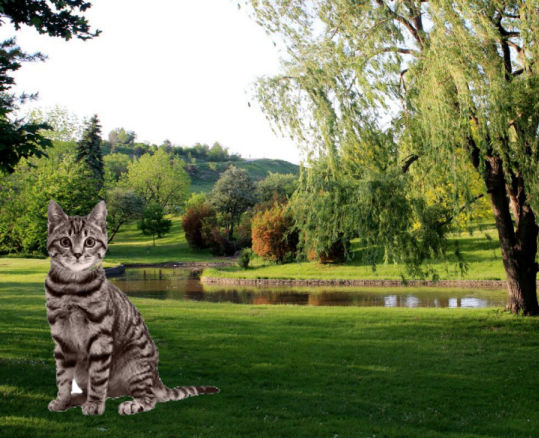
\includegraphics[width=0.24\textwidth]{images/trans_invariance0.png}
    \hspace{0.12\textwidth}
    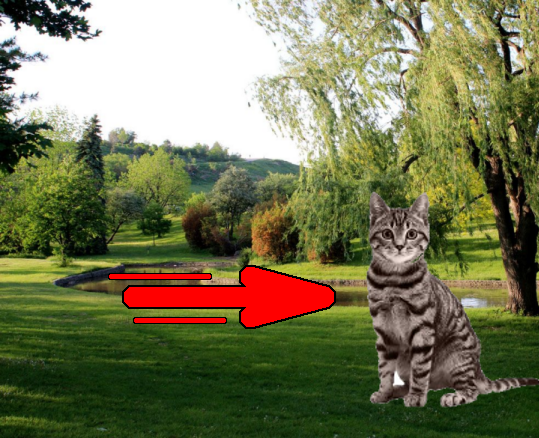
\includegraphics[width=0.24\textwidth]{images/trans_invariance1.png}
    \end{center}
\begin{itemize}
	\item Propriedade interessante de imagens: invariância translacional
    \item Convolução: operador que passa um filtro/kernel/núcleo pequeno por uma imagem para gerar outra imagem
    \item Multiplicação de matrizes está para DFN assim como Convolução está para CNN
\end{itemize}
\end{frame}


\begin{frame}{Aplicando filtros em uma imagem}
\begin{figure}[ht!]
\centering

\scalebox{0.70}{
\begin{tikzpicture}[auto]

% operations =============================

% nodes
\node (original)
    {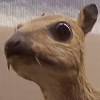
\includegraphics[width=.15\textwidth]{images/Vd-Orig.png}};
\node[above right= 20pt and 150pt of original] (edge) {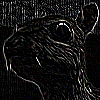
\includegraphics[width=.15\textwidth]{images/Vd-Edge3.png}};
\node[below=20pt of edge] (sharpen) {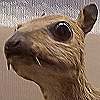
\includegraphics[width=.15\textwidth]{images/Vd-Sharp.png}};
\node[below=20pt of sharpen] (blur) {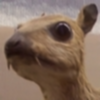
\includegraphics[width=.15\textwidth]{images/Vd-Blur1.png}};

% edges
\path[tedge, orange!120, line width=1mm]  (original) to [out=90,in=180, looseness=9, distance=125pt] (edge);
\path[tedge, orange!120, line width=1mm]  (original) to [out=0,in=180] (sharpen);
\path[tedge, orange!120, line width=1mm]  (original) to [out=-90,in=180, looseness=9, distance=125pt] (blur);

% nodes for kernels 
\node[op3, right=20pt of original] (kernel1) {$\begin{bmatrix}0 & -1 & 0\\ -1 & 5 & -1\\0 & -1 & 0\end{bmatrix}$};
\node[op3, above=10pt of kernel1] (kernel2) {$\begin{bmatrix}-1 & -1 & -1\\ -1 & 8 & -1\\-1 & -1 & -1\end{bmatrix}$};
\node[op3, below=10pt of kernel1] (kernel3) {$\frac{1}{16}\begin{bmatrix}1 & 2 & 1\\ 2 & 4 & 2\\1 & 2 & 1\end{bmatrix}$};

\end{tikzpicture}
} % scalebox
\vspace*{-10mm}
\caption{Exemplo de aplicação de filtros em uma imagem (extraído de \url{https://en.wikipedia.org/wiki/Kernel_(image_processing)})}
\end{figure}

\end{frame}


\begin{frame}{Exemplo de imagem (retirado de \cite{{Dumoulin16}})}
\begin{figure}[ht!]
\centering

\scalebox{0.7}{
    \begin{tikzpicture}[scale=1.5,every node/.style={minimum size=2cm}, on grid]
            \draw[fill=blue2,opacity=1.2] (0,0) rectangle (5,5);
            \draw[draw=base03,thick] (0,0) grid (5,5);
	    	\node (00) at (0.5,4.5) {\LARGE 3};
	    	\node (10) at (0.5,3.5) {\LARGE 0};
            \node (20) at (0.5,2.5) {\LARGE 3};
            \node (30) at (0.5,1.5) {\LARGE 2};
            \node (40) at (0.5,0.5) {\LARGE 2};

	    	\node (01) at (1.5,4.5) {\LARGE 3};
	    	\node (11) at (1.5,3.5) {\LARGE 0};
            \node (21) at (1.5,2.5) {\LARGE 1};
            \node (31) at (1.5,1.5) {\LARGE 0};
            \node (41) at (1.5,0.5) {\LARGE 0};

	    	\node (02) at (2.5,4.5) {\LARGE 2};
	    	\node (12) at (2.5,3.5) {\LARGE 1};
            \node (22) at (2.5,2.5) {\LARGE 2};
            \node (32) at (2.5,1.5) {\LARGE 0};
            \node (42) at (2.5,0.5) {\LARGE 0};

	    	\node (03) at (3.5,4.5) {\LARGE 1};
	    	\node (13) at (3.5,3.5) {\LARGE 3};
            \node (23) at (3.5,2.5) {\LARGE 2};
            \node (33) at (3.5,1.5) {\LARGE 2};
            \node (43) at (3.5,0.5) {\LARGE 0};

	    	\node (04) at (4.5,4.5) {\LARGE 0};
	    	\node (14) at (4.5,3.5) {\LARGE 1};
            \node (24) at (4.5,2.5) {\LARGE 3};
            \node (34) at (4.5,1.5) {\LARGE 2};
            \node (44) at (4.5,0.5) {\LARGE 1};
    \end{tikzpicture}
} % scalebox
\end{figure}

\end{frame}

\begin{frame}{Exemplo de filtro (retirado de \cite{{Dumoulin16}})}
\begin{figure}[ht!]
\centering

\scalebox{0.7}{
    \begin{tikzpicture}[scale=1.4,every node/.style={minimum size=1cm}, on grid]
            \draw[fill=base02,opacity=0.4] (0,0) rectangle (3,3);
            \draw[draw=base03,thick] (0,0) grid (3,3);
            \node (00) at (0.5,2.5) {\Large 0};
            \node (01) at (1.5,2.5) {\Large 1};
            \node (02) at (2.5,2.5) {\Large 2};
            \node (10) at (0.5,1.5) {\Large 2};
            \node (11) at (1.5,1.5) {\Large 2};
            \node (12) at (2.5,1.5) {\Large 0};
            \node (20) at (0.5,0.5) {\Large 0};
            \node (21) at (1.5,0.5) {\Large 1};
            \node (22) at (2.5,0.5) {\Large 2};
    \end{tikzpicture}
} % scalebox
\end{figure}

\end{frame}


\begin{frame}{Convolução (retirado de \cite{{Dumoulin16}})}
\begin{center}
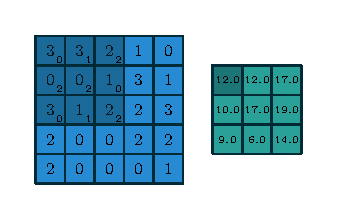
\includegraphics[scale=1.5]{images/numerical_no_padding_no_strides_00.pdf}
\end{center}
\end{frame}

\begin{frame}{Convolução (retirado de \cite{{Dumoulin16}})}
\begin{center}
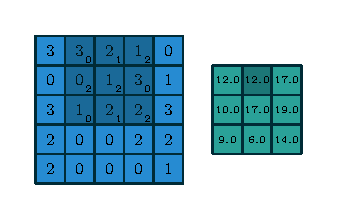
\includegraphics[scale=1.5]{images/numerical_no_padding_no_strides_01.pdf}
\end{center}
\end{frame}

\begin{frame}{Convolução (retirado de \cite{{Dumoulin16}})}
\begin{center}
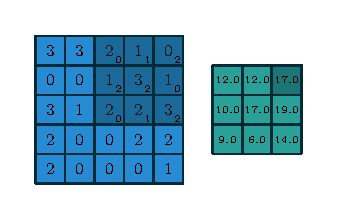
\includegraphics[scale=1.5]{images/numerical_no_padding_no_strides_02.pdf}
\end{center}
\end{frame}



\begin{frame}{Convolução (retirado de \cite{{Dumoulin16}})}
\begin{center}
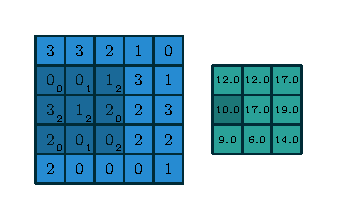
\includegraphics[scale=1.5]{images/numerical_no_padding_no_strides_03.pdf}
\end{center}
\end{frame}

\begin{frame}{Convolução (retirado de \cite{{Dumoulin16}})}
\begin{center}
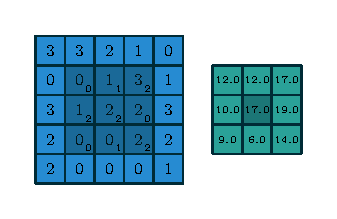
\includegraphics[scale=1.5]{images/numerical_no_padding_no_strides_04.pdf}
\end{center}
\end{frame}

\begin{frame}{Convolução (retirado de \cite{{Dumoulin16}})}
\begin{center}
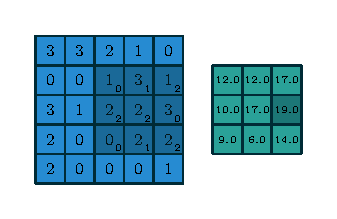
\includegraphics[scale=1.5]{images/numerical_no_padding_no_strides_05.pdf}
\end{center}
\end{frame}

\begin{frame}{Convolução (retirado de \cite{{Dumoulin16}})}
\begin{center}
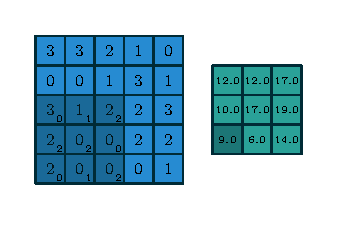
\includegraphics[scale=1.5]{images/numerical_no_padding_no_strides_06.pdf}
\end{center}
\end{frame}


\begin{frame}{Convolução (retirado de \cite{{Dumoulin16}})}
\begin{center}
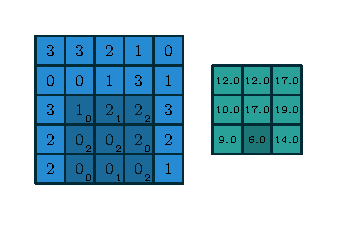
\includegraphics[scale=1.5]{images/numerical_no_padding_no_strides_07.pdf}
\end{center}
\end{frame}

\begin{frame}{Convolução (retirado de \cite{{Dumoulin16}})}
\begin{center}
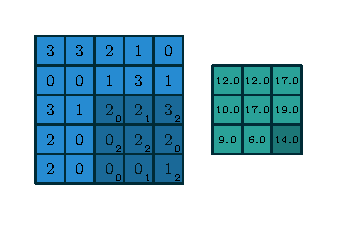
\includegraphics[scale=1.5]{images/numerical_no_padding_no_strides_08.pdf}
\end{center}
\end{frame}

\begin{frame}{Feature map (retirado de \cite{{Dumoulin16}})}
\begin{figure}[ht!]
\centering

\scalebox{0.7}{
    \begin{tikzpicture}[scale=1.4,every node/.style={minimum size=1cm}, on grid]
            \draw[fill=cyan,opacity=1.2] (0,0) rectangle (3,3);
            \draw[draw=base03,thick] (0,0) grid (3,3);
            \node (00) at (0.5,2.5) {\large 12.0};
            \node (01) at (1.5,2.5) {\large 12.0};
            \node (02) at (2.5,2.5) {\large 17.0};
            \node (10) at (0.5,1.5) {\large 10.0};
            \node (11) at (1.5,1.5) {\large 17.0};
            \node (12) at (2.5,1.5) {\large 19.0};
            \node (20) at (0.5,0.5) {\large 9.0};
            \node (21) at (1.5,0.5) {\large 6.0};
            \node (22) at (2.5,0.5) {\large 14.0};
    \end{tikzpicture}
} % scalebox
\end{figure}

\end{frame}


\begin{frame}{Feature map}
Para calcular o tamanho do feature map nos usamos a equação:

\begin{equation*}
 o = (i - k) +1
\end{equation*}


Em que $o \times o$ é o tamanho do feature map, a imagem de entrada tem o tamanho $i \times i$, o tamanho do filtro é $k \times k$, andamos apenas um pixel por vez em cada eixo (\textbf{stride} $= 1$) e não usamos \textbf{padding}.
\end{frame}

\begin{frame}{Same Padding (retirado de \cite{{Dumoulin16}})}
\begin{center}
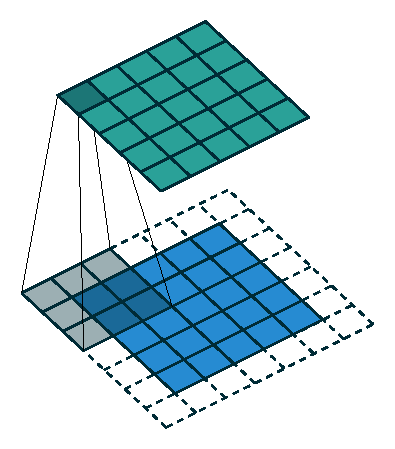
\includegraphics[scale=1]{images/same_padding_no_strides_00.pdf}
\end{center}
\end{frame}

\begin{frame}{Same Padding (retirado de \cite{{Dumoulin16}})}
\begin{center}
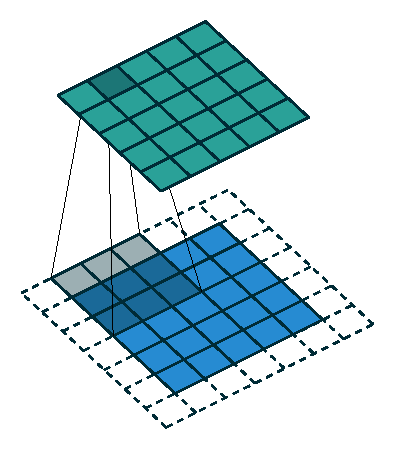
\includegraphics[scale=1]{images/same_padding_no_strides_01.pdf}
\end{center}
\end{frame}

\begin{frame}{Same Padding (retirado de \cite{{Dumoulin16}})}
\begin{center}
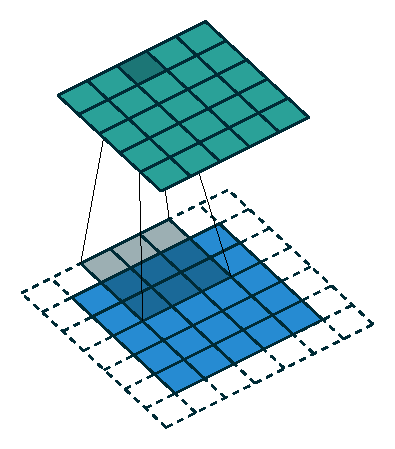
\includegraphics[scale=1]{images/same_padding_no_strides_02.pdf}
\end{center}
\end{frame}

\begin{frame}{Same Padding (retirado de \cite{{Dumoulin16}})}
\begin{center}
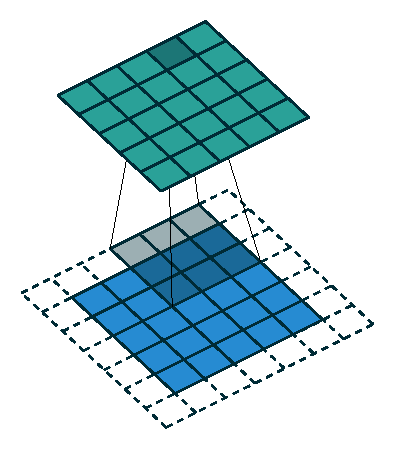
\includegraphics[scale=1]{images/same_padding_no_strides_03.pdf}
\end{center}
\end{frame}


\begin{frame}{Pooling}
\begin{itemize}
\item  Inserimos uma camada de \textbf{pooling} entre camadas de convolução.
\vspace{0.3cm}
\item  Fazemos isso para progressivamente diminuir o número de parâmetros.
\end{itemize}
\end{frame}

\begin{frame}{Max Pooling (retirado de \cite{{Dumoulin16}})}
\begin{center}
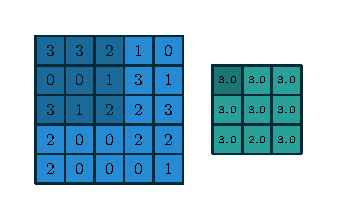
\includegraphics[scale=1.5]{images/numerical_max_pooling_00.pdf}
\end{center}
\end{frame}

\begin{frame}{Max Pooling (retirado de \cite{{Dumoulin16}})}
\begin{center}
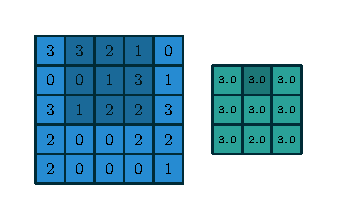
\includegraphics[scale=1.5]{images/numerical_max_pooling_01.pdf}
\end{center}
\end{frame}

\begin{frame}{Max Pooling (retirado de \cite{{Dumoulin16}})}
\begin{center}
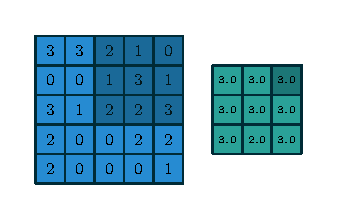
\includegraphics[scale=1.5]{images/numerical_max_pooling_02.pdf}
\end{center}
\end{frame}

\begin{frame}{Max Pooling (retirado de \cite{{Dumoulin16}})}
\begin{center}
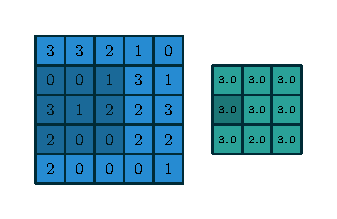
\includegraphics[scale=1.5]{images/numerical_max_pooling_03.pdf}
\end{center}
\end{frame}

\begin{frame}{Max Pooling (retirado de \cite{{Dumoulin16}})}
\begin{center}
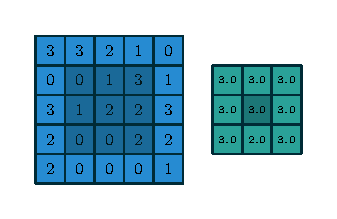
\includegraphics[scale=1.5]{images/numerical_max_pooling_04.pdf}
\end{center}
\end{frame}

\begin{frame}{Max Pooling (retirado de \cite{{Dumoulin16}})}
\begin{center}
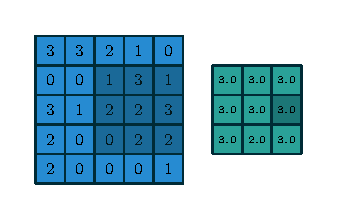
\includegraphics[scale=1.5]{images/numerical_max_pooling_05.pdf}
\end{center}
\end{frame}

\begin{frame}{Max Pooling (retirado de \cite{{Dumoulin16}})}
\begin{center}
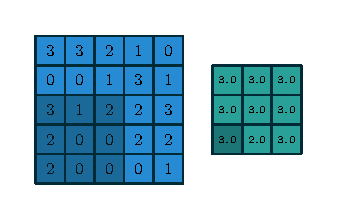
\includegraphics[scale=1.5]{images/numerical_max_pooling_06.pdf}
\end{center}
\end{frame}

\begin{frame}{Max Pooling (retirado de \cite{{Dumoulin16}})}
\begin{center}
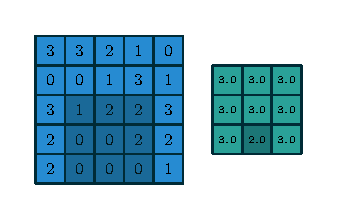
\includegraphics[scale=1.5]{images/numerical_max_pooling_07.pdf}
\end{center}
\end{frame}

\begin{frame}{Max Pooling (retirado de \cite{{Dumoulin16}})}
\begin{center}
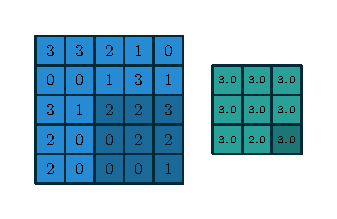
\includegraphics[scale=1.5]{images/numerical_max_pooling_08.pdf}
\end{center}
\end{frame}

\begin{frame}[fragile]{Arquitetura de CNN}
\begin{center}
\begin{tikzpicture}
\node (convlayer) at (0, 0) {CONV};
\node (poollayer) at (1.5, 0) {POOL};
\node (actvlayer) at (3, 0) {ReLU};
\node (otherlayer) at (4.5, 0) {(...)};
\node (fullyconnected) at (6, 0) {FC};
\draw [->, thin] (convlayer.east) -- (poollayer.west);
\draw [->, thin] (poollayer.east) -- (actvlayer.west);
\draw [->, thin] (actvlayer.east) -- (otherlayer.west);
\draw [->, thin] (otherlayer.east) -- (fullyconnected.west);
\end{tikzpicture}
\end{center}
\begin{itemize}
	\item Layers Convolucionais: filtros aprendíveis
    \vspace{1em}
    \item Pooling: reduz a dimensão da imagem
    \vspace{1em}
    \item Ativação: igual à DFN
    \vspace{1em}
    \item Fully-Connected: DFN 
\end{itemize}
\end{frame}

\section{Parte Prática}

\begin{frame}{Tutorial}
Preparamos tutoriais básicos em \textbf{Tensorflow} e \textbf{Keras}:
\vspace{0.3cm}
\begin{center}
\url{https://github.com/MLIME/12aMostra}
\end{center}

\vspace{0.3cm}

\alert{Esses slides também estão lá.}

\end{frame}

\begin{frame}[allowframebreaks]{References}

  \bibliography{my_references}
  \bibliographystyle{abbrv}

\end{frame}

\end{document}
